\documentclass[dvipsnames,handout]{beamer} % Use handout option to remove pauses.
\usetheme{default}
\usefonttheme{structurebold}
\usefonttheme[onlymath]{serif}
\usepackage[UKenglish,cleanlook]{isodate}                                  % Set default date and date display
\usepackage[T1]{fontenc}
% Slide title background color
\definecolor{background}{HTML}{ede6d8}
% Slide title text color
\definecolor{titleText}{HTML}{B40404}
% Add slide numbers in bottom right corner
\defbeamertemplate{headline}{my header}{
    \vskip1pt
    \makebox[0pt][l]{\,\insertsection}
    \hspace*{\fill}\insertshorttitle\hspace*{\fill}
    \llap{\insertframenumber\,/\,\inserttotalframenumber\,}
}
\setbeamertemplate{headline}[my header]
% Add name at the bottom
\setbeamercolor{footlinecolor}{fg=black,bg=background}
\defbeamertemplate{footline}{my footer}{%
    \begin{beamercolorbox}[wd=\paperwidth,leftskip=0.25cm,rightskip=0.25cm]{footlinecolor}
        \insertshortauthor
        \hfill
        \insertframenumber{} / \inserttotalframenumber
    \end{beamercolorbox}
}
\setbeamertemplate{footline}[my footer]
\setbeamertemplate{navigation symbols}[default]
\usepackage{graphicx}
% Set font sizes for frame title and subtitle
\setbeamerfont{frametitle}{size=\fontsize{15}{16}}
\setbeamerfont{framesubtitle}{size=\small}
% Set left and right text margins
\setbeamersize{text margin left=5mm, text margin right=5mm}
\usepackage{booktabs,multirow}
\usepackage{subcaption}   % Sub figures.
\usepackage{tikz}
\usetikzlibrary{shapes,decorations,decorations.pathreplacing,arrows,calc,arrows.meta,fit,positioning}
\tikzset{
    auto,node distance =1 cm and 1 cm,semithick,
    state/.style ={ellipse, draw, minimum width = 0.7 cm},
    point/.style = {circle, draw, inner sep=0.04cm,fill,node contents={}},
    bidirected/.style={Latex-Latex,dashed},
    el/.style = {inner sep=2pt, align=left, sloped}
}
\usepackage{mathtools}                                                     % Various maths functions
\usepackage{amssymb}                                                       % Various maths functions
\usepackage{amsmath}                                                       % Various maths functions
\usepackage{dsfont}                                                        % Various maths functions
\usepackage{centernot}                                                     % center \not usage
\usepackage{siunitx} \sisetup{round-mode=places, round-precision=3}        % Formalise use of units and numbers among text
\usepackage[normalem]{ulem} % Strike-through package
\renewcommand{\vec}[1]{\boldsymbol{\mathit{#1}}}                           % vector notation shortcut
\newcommand{\mat}[1]{\boldsymbol{\mathit{#1}}}                             % matrix notation shortcut
\DeclarePairedDelimiter\abs{\lvert}{\rvert}                                % absolute value notation shortcut
\DeclarePairedDelimiter\norm{\lVert}{\rVert}                               % norm notation shortcut
\newcommand{\Prob}[1]{\Pr\left( #1 \right)}                         % SHortcut for probability notation
\newcommand{\Probgiven}[2]{\Pr\left( #1 \, \middle\vert \, #2 \right)} % SHortcut for probability notation, given
\newcommand{\E}[2][]{\mathbb{E}_{#1} \left[ #2 \right]}                    % Expectation (with optional subscript) shortcut
\newcommand{\Egiven}[3][]{\mathbb{E}_{#1} \left[ #2 \, \middle\vert \, #3 \right]} % Expectation given (with optional subscript) shortcut
\newcommand{\Var}[2][]{\text{Var}_{#1} \left( #2 \right)}                  % Variation (with optional subscript) shortcut
\newcommand{\Cov}[1]{\text{Cov} \left( #1 \right)}                         % Covariance (with optional subscript) shortcut
\newcommand{\indicator}[1]{\mathds{1}\left\{ #1 \right\}}                  % SHortcut for indicator function
\newcommand{\indep}{\, \raisebox{0.05em}{\rotatebox[origin=c]{90}{$\models$}} \,}% Statistical independence symbol.
\newcommand{\diff}[2][]{\frac{d#1}{d#2}}                                   % SHortcut for differential fraction as a function
\newcommand{\partialdiff}[2][]{\frac{\partial#1}{\partial#2}}              % SHortcut for partial differential fraction as a function
\renewcommand{\hat}[1]{\widehat{#1}}                                       % Default estimator notation is widehat
\renewcommand{\bar}[1]{\overline{#1}}                                      % Make over bar look nicer
\renewcommand{\tilde}[1]{\widetilde{#1}}                                   % Make over tilde look better
% Citations
\usepackage{natbib}                                        % Citation package, see https://en.wikibooks.org/wiki/LaTeX/Bibliography_Management#Natbib
\usepackage{hyperref}                                        % Allow for links across the text, with colour options
\usepackage{setspace}
\settowidth{\leftmargini}{\usebeamertemplate{itemize item}}
\addtolength{\leftmargini}{\labelsep}
\usepackage{soul,color,xcolor} % Text highlighting
\newcommand{\eqhighlight}[2]{\colorbox{#1!50}{$\displaystyle#2$}}
\makeatletter
\let\HL\hl
\renewcommand\hl{%
    \let\set@color\beamerorig@set@color
    \let\reset@color\beamerorig@reset@color
    \HL}
\makeatother
\newcommand{\mathcolorbox}[2]{\colorbox{#1}{$\displaystyle #2$}}
% Set colors
\setbeamercolor{block title}{use=structure,fg=white,bg=structure.fg!75!black}
\setbeamercolor{block body}{parent=normal text,use=block title,bg=block title.bg!10!bg}
\setbeamercovered{transparent}
\setbeamercolor{postit}{fg=black, bg=yellow}
\setbeamercolor{frametitle}{bg=background, fg=titleText}
\setbeamercolor{subtitle}{fg=titleText}
% Command to align text
\renewcommand{\raggedright}{\leftskip=0pt \rightskip=0pt plus 0cm}
% Remove the useless buttons.
\setbeamertemplate{navigation symbols}{}
\useoutertheme[footline=empty,subsection=false]{miniframes}
\useinnertheme{circles}

%-------------------------------------------------------------------------------
% Title Page
%-------------------------------------------------------------------------------
\title{\color{titleText}
    \href{https://raw.githubusercontent.com/shoganhennessy/mediation-natural-experiment/main/mediation-natural-experiment-2025.pdf}{Causal Mediation in Natural Experiments}
}
\author[Senan Hogan-Hennessy, Cornell University]{
    Senan Hogan-Hennessy \\
    Economics Department, Cornell University \\ %\vspace{0.5cm}
    \href{mailto:seh325@cornell.edu}{\textcolor{blue}{seh325@cornell.edu}}
}
\date{} % Date, can be changed to a custom date

%-------------------------------------------------------------------------------
% Opening Slides
\begin{document}
% Justify text through-out.
\raggedright
%-------------------------------------------------------------------------------
%% Title page
\begin{frame}[noframenumbering, plain]
    % Print the title page as the first slide
    \vspace{1.5cm}
    \titlepage
    \begin{center}
        \vspace{-1.5cm}
        
\includegraphics[width=2cm]{presentation-files/cornell}

        %\vspace{0.5cm}
        \vskip0pt plus 1filll
        \par\noindent\rule{\textwidth}{0.4pt}
        Cornell Placement Week \\
        29 September 2025
    \end{center}
\end{frame}
%-------------------------------------------------------------------------------
\section{Introduction}
\begin{frame}
    \frametitle{Intro: Oregon Health Insurance Experiment}
    \vspace{-0.125cm}

    In 2008, Oregon gave access to socialised health insurance by wait-list lottery (Finkelstein et al, 2012).
    
    \vspace{-0.625cm}
    \begin{figure}
        \centering
        \singlespacing
        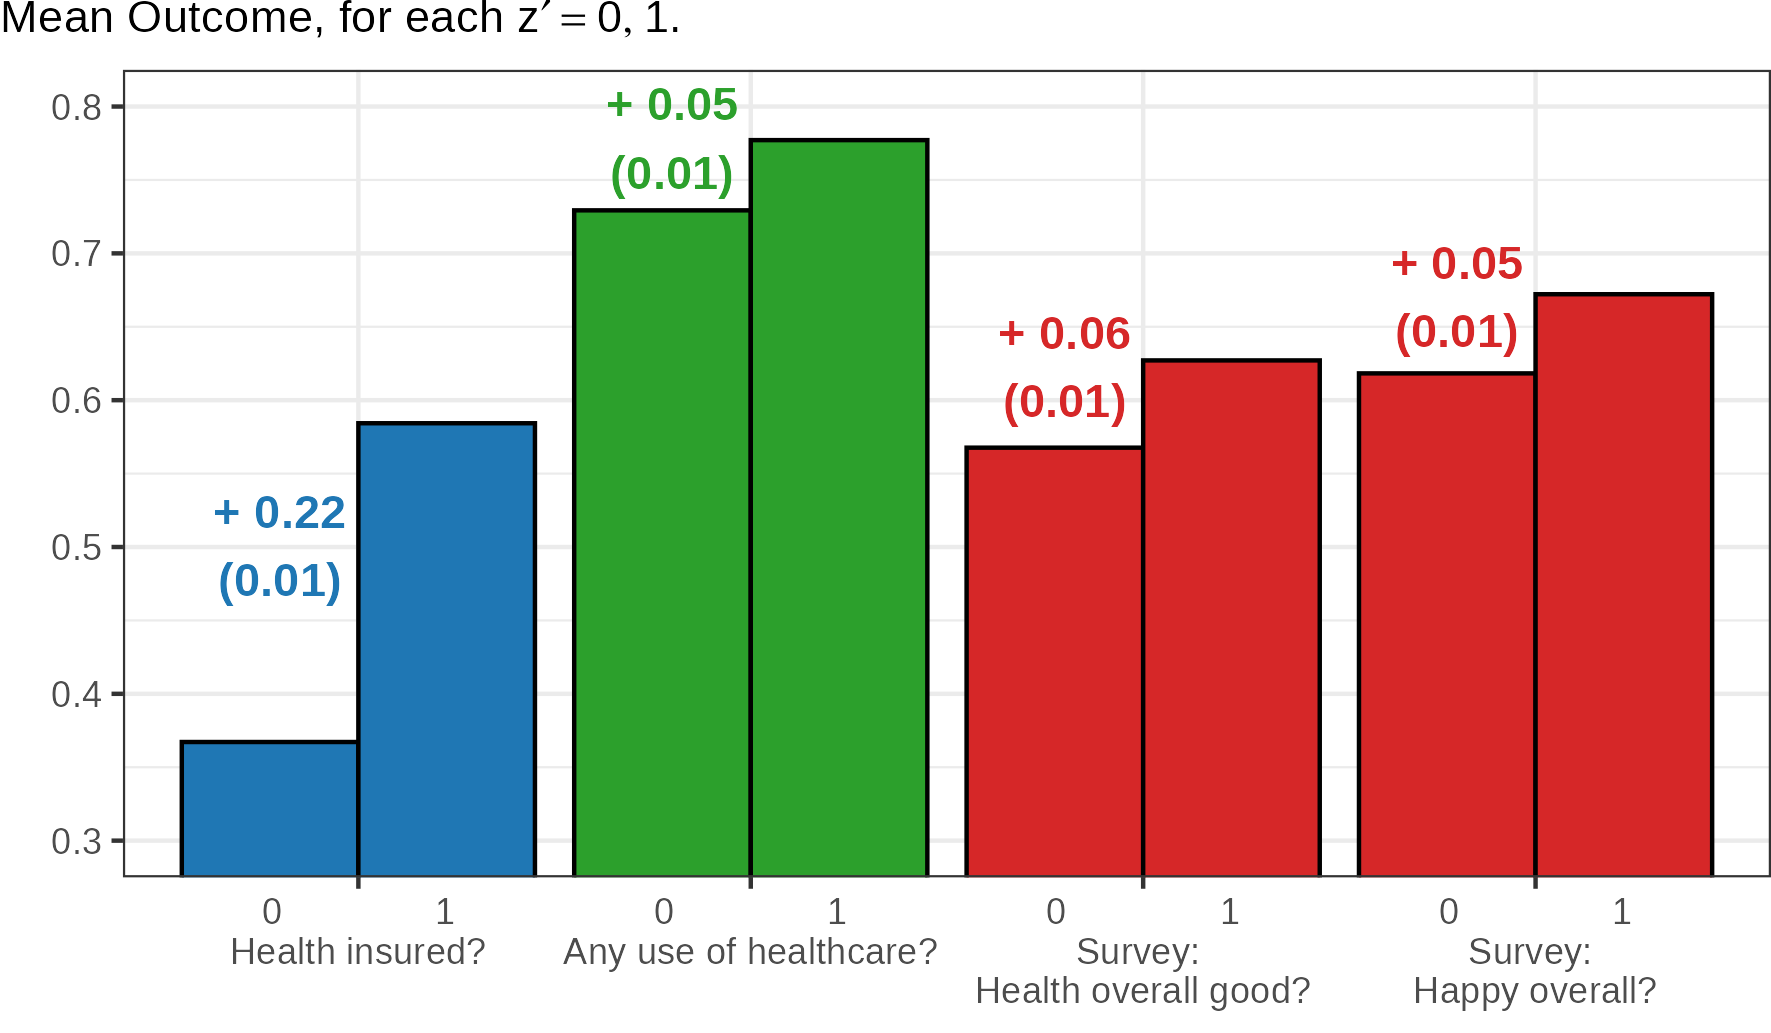
\includegraphics[width=0.85\textwidth]{
            presentation-files/figures/insurance-effects.png}
    \end{figure}
    \vspace{-0.5cm}

    \textbf{Applied practice:}

    $\Rightarrow$ Suggestive evidence for healthcare as mechanism for wait-list lottery….
\end{frame}
%-------------------------------------------------------------------------------
\begin{frame}
    \frametitle{Intro: Oregon Health Insurance Experiment}
    In 2008, Oregon gave access to socialised health insurance by wait-list lottery (Finkelstein et al, 2012).
    \begin{figure}
            \caption{Model for Suggestive Evidence of a Mechanism.}
            
\begin{tikzpicture}
            \node[state,thick,ForestGreen] (mediator) at (0,0) {$D_i$};
            \node[state,thick,blue] (treatment) [left=2cm of mediator] {$Z_i$};
            \node[state,thick,red] (outcome)   [right=2cm of mediator] {$Y_i$};
            % Label Z_i, D, Y_i
            \node[color=ForestGreen] [above=0.1cm of mediator] {Healthcare};
            \node[color=blue] [left=0.1cm of treatment] {Wait-list lottery};
            \node[color=red,align=left] [right=0.1cm of outcome] {Subjective \\ health};
            % Draw the causal arrows
            \path[->, thick] (treatment) edge (mediator);
            %\path[->, dashed,color=gray] (mediator) edge (outcome);
            \path[->, thick] (treatment) edge[bend right=30] (outcome);
            % Label the problem.
            \node[color=RoyalPurple] [right=0.75cm of mediator] {?};
        \end{tikzpicture}
    \end{figure}
    
    \vfill
    \par\noindent\rule{\textwidth}{0.4pt}
    \textbf{Inconsistencies in suggestive evidence of mechanisms:}
    \begin{itemize}
        \item Is $\textcolor{ForestGreen}{D_i} \to \textcolor{red}{Y_i}$ small, large, or even existent?
        \item Where else do we accept assumed causal effects without evidence?
    \end{itemize}
\end{frame}
%-------------------------------------------------------------------------------
\begin{frame}
    \frametitle{Introduction ---  Contributions}
    Causal Mediation (CM) is an alternative framework to studying mechanisms, with clear identification and assumptions required.

    \par\noindent\rule{\textwidth}{0.4pt}
    \begin{enumerate}
        \item Problems with conventional approach to CM in observational settings.
        \\ \textbf{[Negative result]}
        \item Recovering valid CM effects, via MTE $+$ control function modelling.
        \\ \textbf{[Positive result]}
    \end{enumerate}

    \par\noindent\rule{\textwidth}{0.4pt}
    New insights from intersection of two fields:
    \begin{itemize}
        \item \textbf{Causal Mediation (CM).}
        \\ \textcolor{gray}{\footnotesize Imai Keele Yamamoto (2010), Fr\"olich Huber (2017), Deuchert Huber Schelker (2019), Huber (2020), Kwon Roth (2024).}
        \item \textbf{Labour theory, Selection-into-treatment, MTEs.}
        \\ \textcolor{gray}{\footnotesize Roy (1951), Heckman (1979), Heckman Honor\'e (1990), Vycatil (2002), Heckman Vycatil (2005), Brinch Mogstad Wiswall (2017), Kline Walters (2019).}
    \end{itemize}
\end{frame}
%-------------------------------------------------------------------------------
\begin{frame}
    \frametitle{Introduction -- CM}
    Consider ignorable \textcolor{blue}{treatment $Z_i = 0, 1$},
    binary \textcolor{ForestGreen}{mediator $D_i = 0, 1$},
    and continuous \textcolor{red}{outcome $Y_i$}.
    \vskip-0.5cm
    \begin{figure}
        \centering
        \singlespacing
        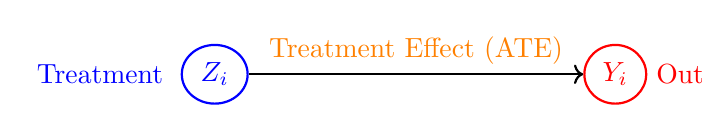
\begin{tikzpicture}
            \node (mediator) at (0,0) {};
            \node[state, thick,blue] (treatment) [left=2cm of mediator] {$Z_i$};
            \node[state, thick,red] (outcome) [right=2cm of mediator] {$Y_i$};
            % Label Z, D, Y
            \node[color=blue] [left=0.1cm of treatment] {Treatment};
            \node[text width=0.1cm, color=red] [right=-0.01cm of outcome] {Outcome};
            % Draw the causal arrows
            \path[->, thick] (treatment) edge (outcome);
            % Label direct and indirect effect
            \node[color=orange] [above=-0.125cm of mediator] {Treatment Effect (ATE)};
        \end{tikzpicture}
    \end{figure}
    
    \vskip0.5cm
    
    \par\noindent\rule{\textwidth}{0.4pt}
    
    \textcolor{gray!25}{
    Assumption:
    \textbf{Mediator Ignorability} (\textbf{MI}, Imai Keele Yamamoto 2010)
    \vskip0.125cm
    mediator $D_i$ is \textit{also} ignorable, conditional on $\vec X_i$ and $Z_i$ realisation.}
    
    \par\noindent\rule{\textwidth}{0.4pt}
    \textcolor{gray!25}{
    Average Direct Effect (ADE) and Average Indirect Effect (AIE) are identified by two-stage regression}
    %\[ \text{Average Direct Effect (ADE)}: \;\;\;
    %    \E{Y_i\left(\eqhighlight{blue}{1}, D_i(Z_i) \right)
    %        - Y_i\left(\eqhighlight{blue}{0}, D_i(Z_i) \right)} \]
    %\vskip-0.35cm
    \begin{itemize}
        \item \textcolor{gray!25}{ADE is causal effect $Z_i \to Y_i$, blocking the indirect $D_i$ path}
        \item \textcolor{gray!25}{AIE is causal effect of $D_i(Z_i) \to Y_i$, blocking the direct $Z_i$ path.}
    \end{itemize}
    %\[ \text{Average Indirect Effect (AIE):} \;\;\;
    %\E{Y_i\left(Z_i, \eqhighlight{ForestGreen}{D_i(1)} \right)
    %    - Y_i\left(Z_i, \eqhighlight{ForestGreen}{D_i(0)} \right)} \]
    %\vskip-0.25cm
\end{frame}
%-------------------------------------------------------------------------------
\begin{frame}[noframenumbering]
    \frametitle{Introduction -- CM}
    Consider ignorable \textcolor{blue}{treatment $Z_i = 0, 1$},
    binary \textcolor{ForestGreen}{mediator $D_i = 0, 1$},
    and continuous \textcolor{red}{outcome $Y_i$}.
    \vskip-0.75cm
    \begin{figure}
        \centering
        \singlespacing
        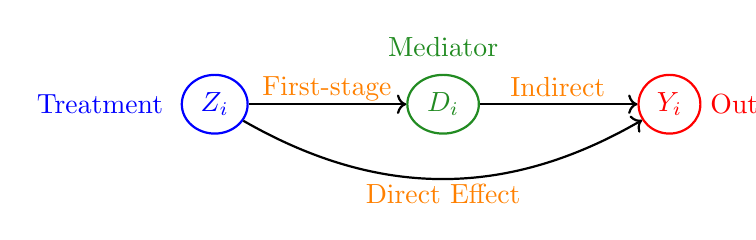
\begin{tikzpicture}
            \node[state, thick,ForestGreen] (mediator) at (0,0) {$D_i$};
            \node[state, thick,blue] (treatment) [left=2cm of mediator] {$Z_i$};
            \node[state, thick,red] (outcome) [right=2cm of mediator] {$Y_i$};
            % Label Z, D, Y
            \node[color=ForestGreen] [above=0.1cm of mediator] {Mediator};
            \node[color=blue] [left=0.1cm of treatment] {Treatment};
            \node[text width=0.1cm, color=red] [right=-0.01cm of outcome] {Outcome};
            % Draw the causal arrows
            \path[->, thick] (treatment) edge (mediator);
            \path[->, thick] (mediator) edge (outcome);
            \path[->, thick] (treatment) edge[bend right=30] (outcome);
            % Label direct and indirect effect
            \node[color=orange] [above left=-0.35cm and 0.2cm of mediator] {First-stage};
            \node[color=orange] [above right=-0.3cm and 0.4cm of mediator] {Indirect};
            \node[color=orange] [below=0.5cm of mediator] {Direct Effect};
        \end{tikzpicture}
    \end{figure}
    \pause
    \vskip-0.25cm
    \par\noindent\rule{\textwidth}{0.4pt}
    Assumption:
    \textbf{Mediator Ignorability} (\textbf{MI}, Imai Keele Yamamoto 2010)
    \vskip0.125cm
    \textcolor{ForestGreen}{mediator $D_i$} is \textit{also} ignorable, conditional on $\vec X_i$ and \textcolor{blue}{$Z_i$ realisation}.
    
    \par\noindent\rule{\textwidth}{0.4pt}
    Average Direct Effect (ADE) and Average Indirect Effect (AIE) are identified by two-stage regression
    %\[ \text{Average Direct Effect (ADE)}: \;\;\;
    %    \E{Y_i\left(\eqhighlight{blue}{1}, D_i(Z_i) \right)
    %        - Y_i\left(\eqhighlight{blue}{0}, D_i(Z_i) \right)} \]
    %\vskip-0.35cm
    \begin{itemize}
        \item ADE is causal effect $\textcolor{blue}{Z_i} \to Y_i$, blocking the indirect $D_i$ path
        \item AIE is causal effect of $\textcolor{ForestGreen}{D_i(Z_i)} \to Y_i$, blocking the direct $Z_i$ path.
    \end{itemize}
    %\[ \text{Average Indirect Effect (AIE):} \;\;\;
    %\E{Y_i\left(Z_i, \eqhighlight{ForestGreen}{D_i(1)} \right)
    %    - Y_i\left(Z_i, \eqhighlight{ForestGreen}{D_i(0)} \right)} \]
    %\vskip-0.25cm
\end{frame}
%-------------------------------------------------------------------------------
\section{1. Selection Bias}
%-------------------------------------------------------------------------------
\begin{frame}
    \frametitle{1. Selection Bias}
    Assumption:
    \textbf{Mediator ignorability} (\textbf{MI}, Imai Keele Yamamoto 2010)
    \vskip0.125cm
    \textcolor{ForestGreen}{mediator $D_i$} is \textbf{\textit{also} ignorable}, conditional on $\vec X_i$, \textcolor{blue}{$Z_i$ realisation}
    %\[ D_i \indep Y_i(z', d') \;\; | \;\; \vec X_i, Z_i = z',
    %    \text{ for } z', d' = 0, 1. \]
    %\vskip-0.25cm
    \par\noindent\rule{\textwidth}{0.4pt}
    \colorbox{yellow}{Would this assumption hold true in settings economists study?}

    \vskip0.25cm    
    E.g., Oregon Health Insurance Experiment.
    \begin{figure}
        
\begin{tikzpicture}
            \node[state,thick,ForestGreen] (mediator) at (0,0) {$D_i$};
            \node[state,thick,blue] (treatment) [left=2cm of mediator] {$Z_i$};
            \node[state,thick,red] (outcome)   [right=2cm of mediator] {$Y_i$};
            % Label Z_i, D, Y_i
            \node[color=ForestGreen] [above=0.1cm of mediator] {Healthcare};
            \node[color=blue] [left=0.1cm of treatment] {Wait-list lottery};
            \node[color=red,align=left] [right=0.1cm of outcome] {Subjective \\ health};
            % Draw the causal arrows
            \path[->, thick] (treatment) edge (mediator);
            \path[->, thick] (mediator) edge (outcome);
            \path[->, thick] (treatment) edge[bend right=30] (outcome);
        \end{tikzpicture}
    \end{figure}
    \begin{enumerate}
        \item Treatment is as-good-as random (2008 Oregon wait-list lottery).
        \item \colorbox{yellow}{Healthcare is quasi-random, conditional on lottery realisation $Z_i$} \\
        \colorbox{yellow}{and demographic controls $\vec X_i$.}
    \end{enumerate}
\end{frame}
%-------------------------------------------------------------------------------
\begin{frame}
    \frametitle{1. Selection Bias}
    Assumption: \textbf{Mediator ignorability} (\textbf{MI}, Imai Keele Yamamoto 2010)
    \vskip0.125cm
    \textcolor{ForestGreen}{mediator $D_i$} is \textbf{\textit{also} ignorable}, conditional on $\vec X_i$, \textcolor{blue}{$Z_i$ realisation}
    %\[ D_i \indep Y_i(z', d') \;\; | \;\; \vec X_i, Z_i = z',
    %    \text{ for } z', d' = 0, 1. \]
    %\vskip-0.25cm
    \par\noindent\rule{\textwidth}{0.4pt}
    \colorbox{yellow}{Would this assumption hold true in settings economists study?}

    \vskip0.25cm    
    E.g., Oregon Health Insurance Experiment.
    \vskip-0.75cm
    \begin{figure}
        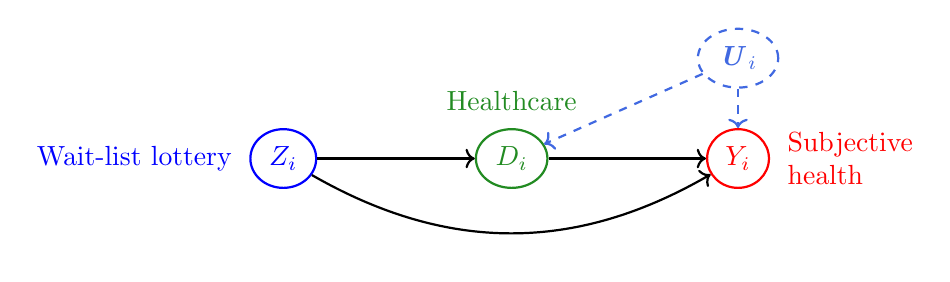
\begin{tikzpicture}
            \node[state,thick,ForestGreen] (mediator) at (0,0) {$D_i$};
            \node[state,thick,blue] (treatment) [left=2cm of mediator] {$Z_i$};
            \node[state,thick,red] (outcome)   [right=2cm of mediator] {$Y_i$};
            % Label Z_i, D, Y_i
            \node[color=ForestGreen] [above=0.1cm of mediator] {Healthcare};
            \node[color=blue] [left=0.1cm of treatment] {Wait-list lottery};
            \node[color=red,align=left] [right=0.1cm of outcome] {Subjective \\ health};
            % Draw the causal arrows
            \path[->, thick] (treatment) edge (mediator);
            \path[->, thick] (mediator) edge (outcome);
            \path[->, thick] (treatment) edge[bend right=30] (outcome);
            \pause
            \node[state, thick,dashed,thick,RoyalBlue] (confounderU) [
                above=0.5cm of outcome] {$\vec U_i$};
            \path[->,thick,dashed,color=RoyalBlue] (confounderU) edge (mediator);
            \path[->,thick,dashed,color=RoyalBlue] (confounderU) edge (outcome);

        \end{tikzpicture}
    \end{figure}
    \textbf{Theorem:}
    If choice to attend healthcare is unconstrained, based on costs and benefits (Roy model) and demographics do not explain all benefits $\implies$ \textbf{MI} does not hold, there is unobserved confounding.
\end{frame}
%-------------------------------------------------------------------------------
% \begin{frame}
%     \frametitle{1. Selection Bias}
%     In an observational setting, need an additional credible research design for \textbf{Mediator Ignorability (MI)} to be credible.
%     \vskip-0.5cm
%     \begin{figure}[h!]
%         \centering
%         \singlespacing
%         \begin{subfigure}[c]{0.475\textwidth}
%             \centering
%             \caption{Cells in a lab
%                 $\to$ \textbf{MI} believable.}
%             
\includegraphics[width=\textwidth]{presentation-files/figures/science-lab.png}
%         \end{subfigure}
%         \begin{subfigure}[c]{0.475\textwidth}
%             \centering
%             \caption{People choosing healthcare
%                 $\to$ \textbf{MI} not.}
%             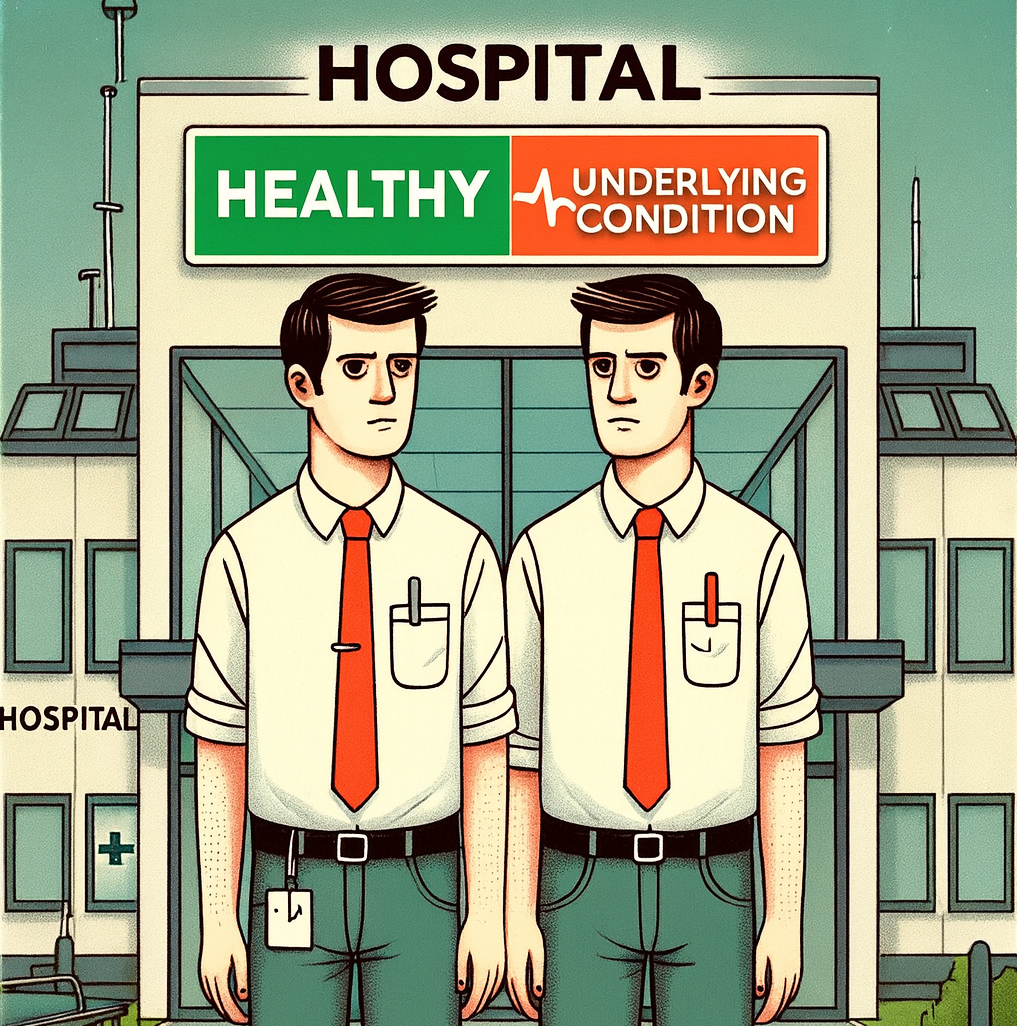
\includegraphics[width=0.965\textwidth]{presentation-files/figures/health-differences.png}
%         \end{subfigure}
%     \end{figure}
% \end{frame}
%-------------------------------------------------------------------------------
\begin{frame}
    \frametitle{1. Selection Bias}
    \label{main:selection-bias}
    In an observational setting, need an additional credible research design for \textbf{Mediator Ignorability (MI)} to be credible.
    \vskip-0.5cm
    \begin{figure}
        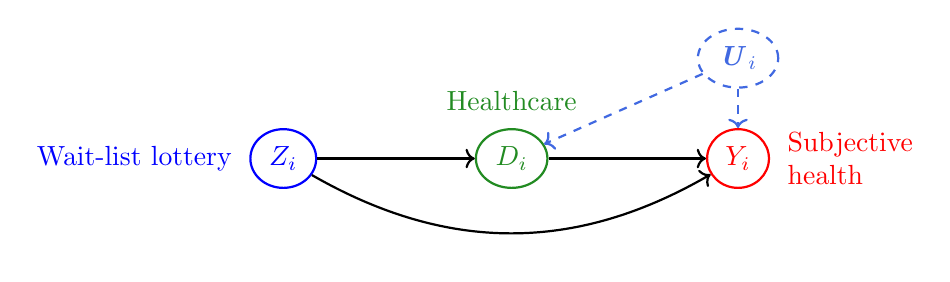
\begin{tikzpicture}
            \node[state,thick,ForestGreen] (mediator) at (0,0) {$D_i$};
            \node[state,thick,blue] (treatment) [left=2cm of mediator] {$Z_i$};
            \node[state,thick,red] (outcome)   [right=2cm of mediator] {$Y_i$};
            % Label Z_i, D, Y_i
            \node[color=ForestGreen] [above=0.1cm of mediator] {Healthcare};
            \node[color=blue] [left=0.1cm of treatment] {Wait-list lottery};
            \node[color=red,align=left] [right=0.1cm of outcome] {Subjective \\ health};
            % Draw the causal arrows
            \path[->, thick] (treatment) edge (mediator);
            \path[->, thick] (mediator) edge (outcome);
            \path[->, thick] (treatment) edge[bend right=30] (outcome);
            \node[state, thick,dashed,thick,RoyalBlue] (confounderU) [
                above=0.5cm of outcome] {$\vec U_i$};
            \path[->,thick,dashed,color=RoyalBlue] (confounderU) edge (mediator);
            \path[->,thick,dashed,color=RoyalBlue] (confounderU) edge (outcome);
        \end{tikzpicture}
    \end{figure}
    \vskip-0.5cm
    \par\noindent\rule{\textwidth}{0.4pt}
    \pause
    If not, then CM effects are contaminated by bias terms, similar to classical selection bias \textcolor{gray}{(e.g., Heckman Ichimura Smith Todd 1998)}.
    %\hyperlink{cm-model}{\beamergotobutton{Model}}
    \begin{itemize}
        \item ADE:
        $ \;\;\ \text{\textcolor{purple}{CM Estimand}}
        = \text{\textcolor{blue}{ADE}}
            + \Big(\text{\textcolor{red}{Selection Bias}}
            + \text{\textcolor{orange}{Group difference bias}}\Big) $
        \item AIE:
        $ \;\;\;\; \text{\textcolor{purple}{CM Estimand}}
            = \text{\textcolor{ForestGreen}{AIE}}
            + \Big(\text{\textcolor{red}{Selection Bias}}
            + \text{\textcolor{orange}{Group difference bias}}\Big) $
        \hyperlink{group-diff-ade}{\beamergotobutton{ADE biases}}
        \hfill
        \hyperlink{group-diff-aie}{\beamergotobutton{AIE biases}}
    \end{itemize}
\end{frame}
%-------------------------------------------------------------------------------
\begin{frame}
    \frametitle{1. Selection Bias}
    In a simulation with Roy selection-into-$\textcolor{ForestGreen}{D_i}$, CM estimates are biased.

    \makebox[\textwidth]{\parbox{1.25\textwidth}{
        \begin{figure}
            \vskip-0.25cm
            %\caption{Simulated Distribution of CM Effect Estimates from 10,000 DGPs.}
            %\vskip-0.25cm
            \begin{subfigure}[c]{0.525\textwidth}
                \centering
                \caption{$\hat{\text{ADE}} - \text{ADE}$.}
                \vskip-0.25cm
                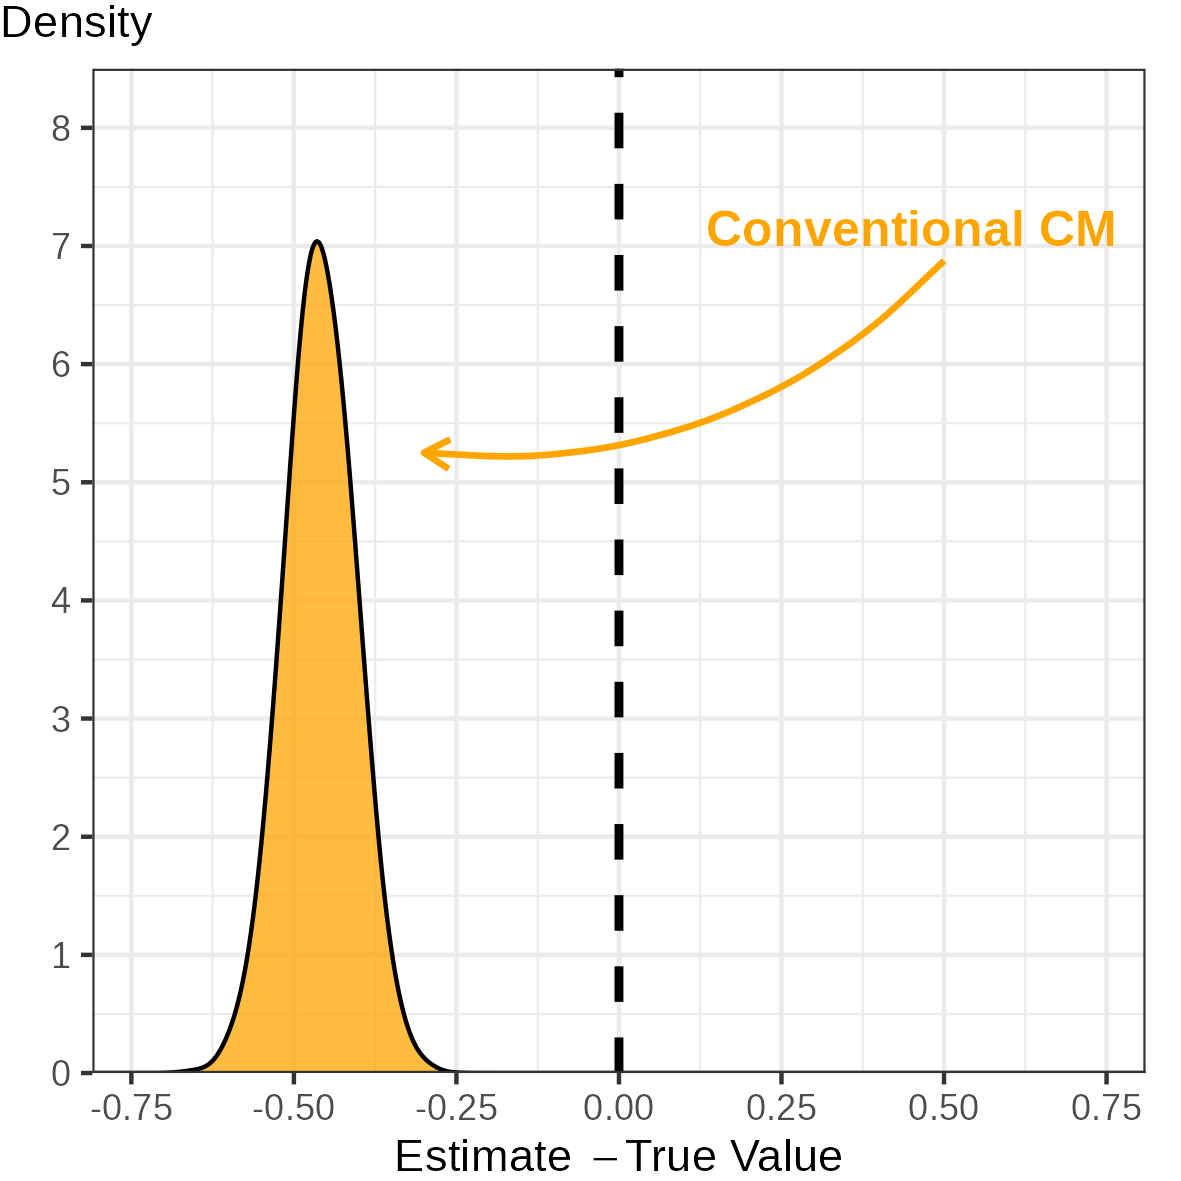
\includegraphics[width=\textwidth]{
                    ../text/sections/figures/ols-direct-dist.png}
            \end{subfigure}
            \begin{subfigure}[c]{0.525\textwidth}
                \centering
                \caption{$\hat{\text{AIE}} - \text{AIE}$.}
                \vskip-0.25cm
                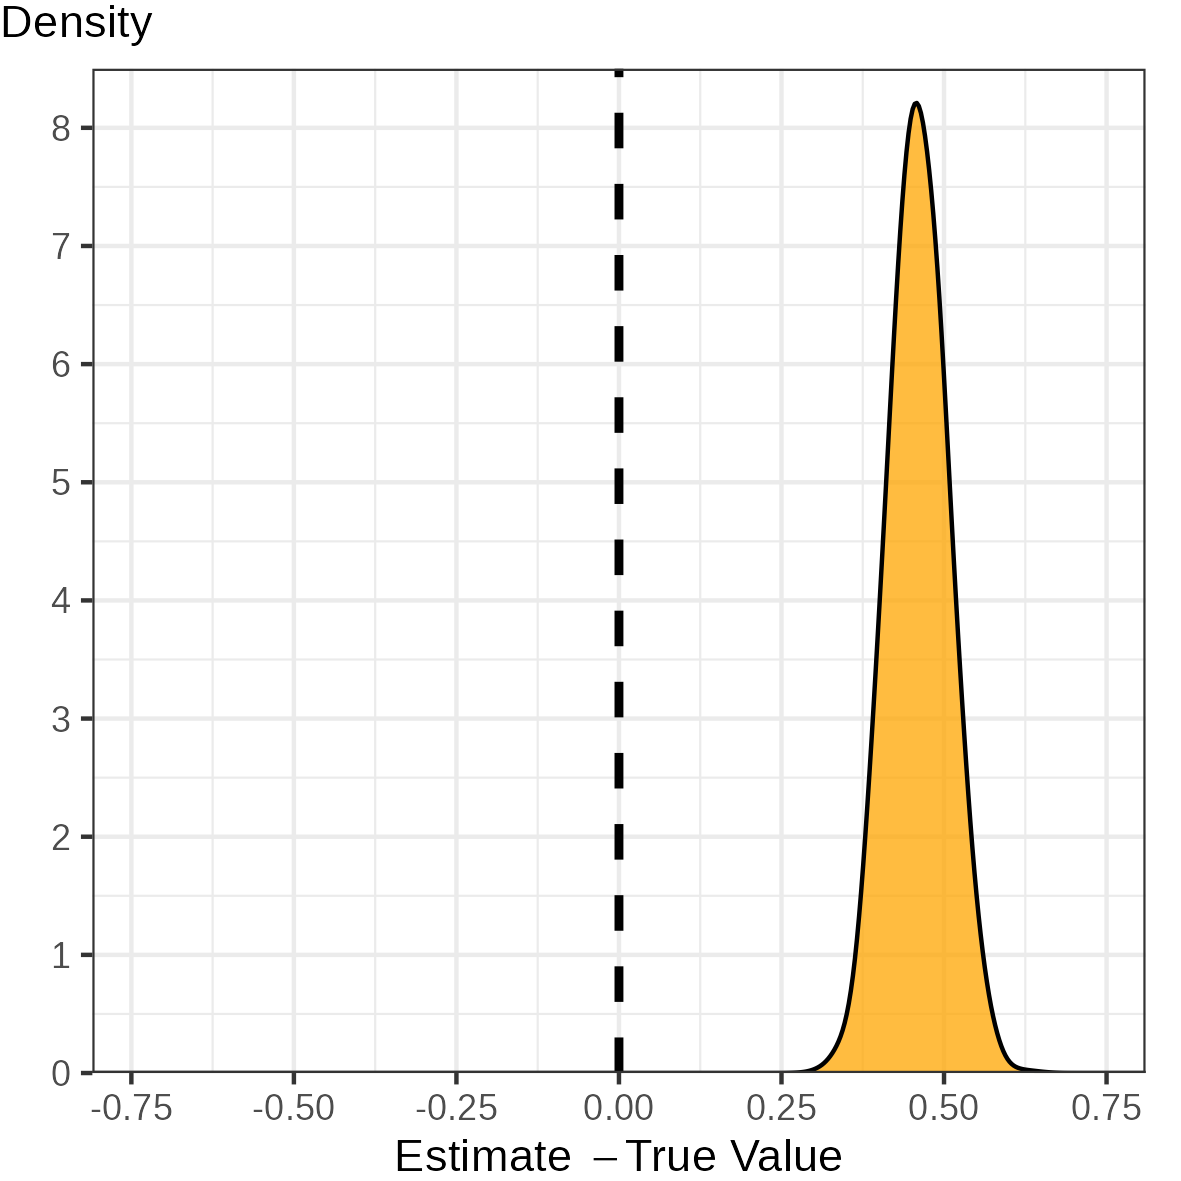
\includegraphics[width=\textwidth]{
                    ../text/sections/figures/ols-indirect-dist.png}
            \end{subfigure}
        \end{figure}
    }}
\end{frame}
%-------------------------------------------------------------------------------
\section{2. CM with Selection}
%-------------------------------------------------------------------------------
\begin{frame}
    \frametitle{2. CM with Selection}
    Conventional CM methods do not identify ADE $+$ AIE in a natural experiment setting, but can we build a credible structural model? 

    \par\noindent\rule{\textwidth}{0.4pt}
    Suppose $\textcolor{blue}{Z_i}$ is ignorable, but $\textcolor{ForestGreen}{D_i}$ is not:

    \vskip-0.75cm
    \begin{figure}
        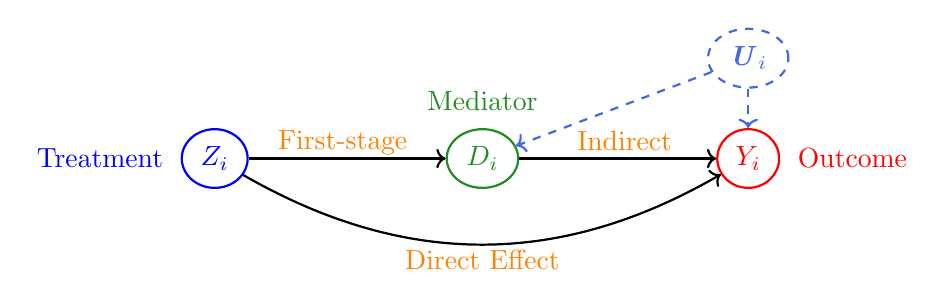
\begin{tikzpicture}
            \node[state,thick,ForestGreen] (mediator) at (0,0) {$D_i$};
            \node[state,thick,blue] (treatment) [left=2.5cm of mediator] {$Z_i$};
            \node[state,thick,red] (outcome)   [right=2.5cm of mediator] {$Y_i$};
            % Label Z_i, D, Y_i
            \node[color=ForestGreen] [above=0.1cm of mediator] {Mediator};
            \node[color=blue] [left=0.1cm of treatment] {Treatment};
            \node[color=red,align=left] [right=0.1cm of outcome] {Outcome};
            % Draw the causal arrows
            \path[->, thick] (treatment) edge (mediator);
            \path[->, thick] (mediator) edge (outcome);
            \path[->, thick] (treatment) edge[bend right=30] (outcome);
            \node[state, thick,dashed,thick,RoyalBlue] (confounderU) [
                above=0.5cm of outcome] {$\vec U_i$};
            \path[->,thick,dashed,color=RoyalBlue] (confounderU) edge (mediator);
            \path[->,thick,dashed,color=RoyalBlue] (confounderU) edge (outcome);
            % Lable direct and indirect effects
            \node[color=orange] [above left=-0.35cm and 0.5cm of mediator] {First-stage};
            \node[color=orange] [above right=-0.3cm and 0.75cm of mediator] {Indirect};
            \node[color=orange] [below=0.65cm of mediator] {Direct Effect};
        \end{tikzpicture}
    \end{figure}
    \vskip-0.5cm

    \par\noindent\rule{\textwidth}{0.4pt}
    
    \begin{enumerate}
        \item Average first-stage, $\textcolor{blue}{Z_i} \to \textcolor{ForestGreen}{D_i}$, is identified
        \item Average second-stage, $\textcolor{blue}{Z_i}, \textcolor{ForestGreen}{D_i} \to \textcolor{red}{Y_i}$, is not --- represented by $\vec U_i$.
    \end{enumerate}
    \vfill
    \textbf{Intuition}:
    model $\vec U_i$ via mediator MTE to identify ADE $+$ AIE.
\end{frame}
%-------------------------------------------------------------------------------
\begin{frame}
    \frametitle{2. CM with Selection --- Identification}
    \begin{columns}[T]
        \begin{column}{0.3\textwidth}
            \textbf{MTE assumptions}:
        \end{column}
        % Column 2    
        \begin{column}{0.6\textwidth}
            \vskip-0.25cm
            \begin{enumerate}
                \item Mediator monotonicity
                \item Selection on mediator benefits
                \item IV for mediator take-up cost.
            \end{enumerate}
        \end{column}
    \end{columns}
    \vskip0.25cm

    \par\noindent\rule{\textwidth}{0.4pt}
    Causal model:

    \vskip-1cm
    \begin{figure}
        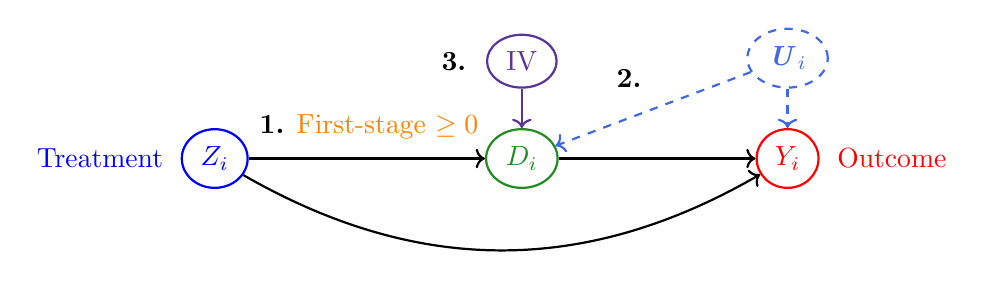
\begin{tikzpicture}
            \node[state,thick,ForestGreen] (mediator) at (0,0) {$D_i$};
            \node[state,thick,blue] (treatment) [left=3cm of mediator] {$Z_i$};
            \node[state,thick,red] (outcome)   [right=2.5cm of mediator] {$Y_i$};
            % Label Z_i, D, Y_i
            %\node[color=ForestGreen] [above=0.1cm of mediator] {Mediator};
            \node[color=blue] [left=0.1cm of treatment] {Treatment};
            \node[color=red,align=left] [right=0.1cm of outcome] {Outcome};
            % Draw the causal arrows
            \path[->, thick] (treatment) edge (mediator);
            \path[->, thick] (mediator) edge (outcome);
            \path[->, thick] (treatment) edge[bend right=30] (outcome);
            \node[state, thick,dashed,thick,RoyalBlue] (confounderU) [
                above=0.5cm of outcome] {$\vec U_i$};
            % Label direct and indirect effects
            %\node[color=orange] [above right=-0.3cm and 0.75cm of mediator] {Indirect};
            %\node[color=orange] [below=0.75cm of mediator] {Direct Effect};
            \pause
            \node[align=left] [above left=-0.15cm and 0.1cm of mediator] {\textbf{1.} \textcolor{orange}{First-stage $\geq 0$}};
            \pause
            \node [above right=0.5cm and 0.75cm of mediator] {\textbf{2.}};
            %\path[->,thick,dashed,color=white] (confounderU) edge (mediator);
            %\path[->,thick,dashed,color=RoyalBlue] (confounderU) edge (mediator);
            \path[->,thick,dashed,color=RoyalBlue] (confounderU) edge (mediator);
            \path[->,thick,dashed,color=RoyalBlue] (confounderU) edge (outcome);
            \pause
            \node[state,thick,RoyalPurple] (instrument) [above=0.5cm of mediator] {IV};
            \path[->,thick,color=RoyalPurple] (instrument) edge (mediator);
            \node [left=0.125cm of instrument] {\textbf{3.}};
        \end{tikzpicture}
    \end{figure}

    
    \vskip-0.75cm

    \par\noindent\rule{\textwidth}{0.4pt}
    \textbf{Proposition:}
    Under MTE assumptions, the mediator MTE is identified.
    \vskip0.5cm

    \pause
    \textbf{Theorem}:
    Mediation second-stage effects, $\textcolor{blue}{Z_i}, \textcolor{ForestGreen}{D_i} \to \textcolor{red}{Y_i}$, are identified by the MTE associated Control Functions (CFs).
\end{frame}
%-------------------------------------------------------------------------------
\begin{frame}
    \frametitle{2. CM with Selection --- Identification}
    \begin{columns}[T]
        \begin{column}{0.3\textwidth}
            \textbf{MTE assumptions}:
        \end{column}
        % Column 2    
        \begin{column}{0.6\textwidth}
            \vskip-0.25cm
            \begin{enumerate}
                \item Mediator monotonicity
                \item Selection on mediator benefits
                \item IV for mediator take-up cost.
            \end{enumerate}
        \end{column}
    \end{columns}
    \vskip0.25cm

    \par\noindent\rule{\textwidth}{0.4pt}
    Causal model:

    \vskip-1cm
    \begin{figure}
        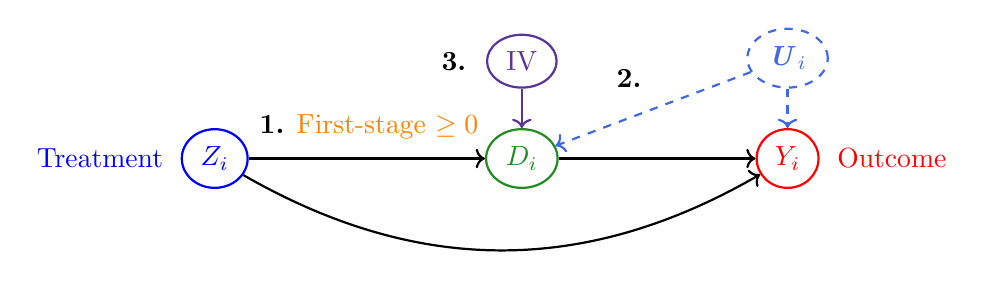
\begin{tikzpicture}
            \node[state,thick,ForestGreen] (mediator) at (0,0) {$D_i$};
            \node[state,thick,blue] (treatment) [left=3cm of mediator] {$Z_i$};
            \node[state,thick,red] (outcome)   [right=2.5cm of mediator] {$Y_i$};
            % Label Z_i, D, Y_i
            %\node[color=ForestGreen] [above=0.1cm of mediator] {Mediator};
            \node[color=blue] [left=0.1cm of treatment] {Treatment};
            \node[color=red,align=left] [right=0.1cm of outcome] {Outcome};
            % Draw the causal arrows
            \path[->, thick] (treatment) edge (mediator);
            \path[->, thick] (mediator) edge (outcome);
            \path[->, thick] (treatment) edge[bend right=30] (outcome);
            \node[state, thick,dashed,thick,RoyalBlue] (confounderU) [
                above=0.5cm of outcome] {$\vec U_i$};
            % Label direct and indirect effects
            %\node[color=orange] [above right=-0.3cm and 0.75cm of mediator] {Indirect};
            %\node[color=orange] [below=0.75cm of mediator] {Direct Effect};
            \node[align=left] [above left=-0.15cm and 0.1cm of mediator] {\textbf{1.} \textcolor{orange}{First-stage $\geq 0$}};
            \node [above right=0.5cm and 0.75cm of mediator] {\textbf{2.}};
            %\path[->,thick,dashed,color=white] (confounderU) edge (mediator);
            %\path[->,thick,dashed,color=RoyalBlue] (confounderU) edge (mediator);
            \path[->,thick,dashed,color=RoyalBlue] (confounderU) edge (mediator);
            \path[->,thick,dashed,color=RoyalBlue] (confounderU) edge (outcome);
            \node[state,thick,RoyalPurple] (instrument) [above=0.5cm of mediator] {IV};
            \path[->,thick,color=RoyalPurple] (instrument) edge (mediator);
            \node [left=0.125cm of instrument] {\textbf{3.}};
        \end{tikzpicture}
    \end{figure}

    
    \vskip-0.75cm

    \par\noindent\rule{\textwidth}{0.4pt}
    \textbf{Proposition:}
    Under MTE assumptions, the mediator MTE is identified.
    \vskip0.5cm

    \pause
    \textbf{Intuition:}
    Identifies ADE $+$ AIE by extrapolating from IV compliers to mediator compliers
    \textcolor{gray}{(MTE extrapolation e.g., Mogstad Torgovitsky 2018)}.
\end{frame}
%-------------------------------------------------------------------------------
\begin{frame}
    \frametitle{2. CM with Selection --- Estimation}
    In practice, this means two-stage CM estimation, with CF in second-stage.

    \par\noindent\rule{\textwidth}{0.4pt}
    \textbf{Parametric CF Estimation Recipe:}
    \begin{enumerate}
        \item Estimate mediation first-stage with probit, including the IV.
        \item Estimate mediation second-stage by OLS, with Mills ratio CF terms (Heckman 1979).
        \item Compose CM estimates from two-stage plug-in estimates
        \\(same as parametric MTEs, Bj{\"o}rklund Moffitt 1987).
    \end{enumerate}

    \vskip0.5cm
    \textcolor{gray!25}{
        \textbf{Semi-parametric CF Estimation Recipe:} \\
        Replace \textbf{2.} with semi-parametric CFs
        (same estimation as MTEs).}

    \vfill

    \par\noindent\rule{\textwidth}{0.4pt}
    $\implies$ Conventional CM estimates (two-stages) $+$ IV-guided CF adjustment.
\end{frame}
%-------------------------------------------------------------------------------
\begin{frame}
    \frametitle{2. CM with Selection --- Estimation}
    \vskip-0.25cm
    \makebox[\textwidth]{\parbox{1.25\textwidth}{
        \begin{figure}
            \caption{CM Estimates from 10,000 DGPs with \textbf{Normal} Errors.}
            \vskip-0.25cm
            \begin{subfigure}[c]{0.525\textwidth}
                \centering
                \caption{$\hat{\text{ADE}} - \text{ADE}$.}
                \vskip-0.25cm
                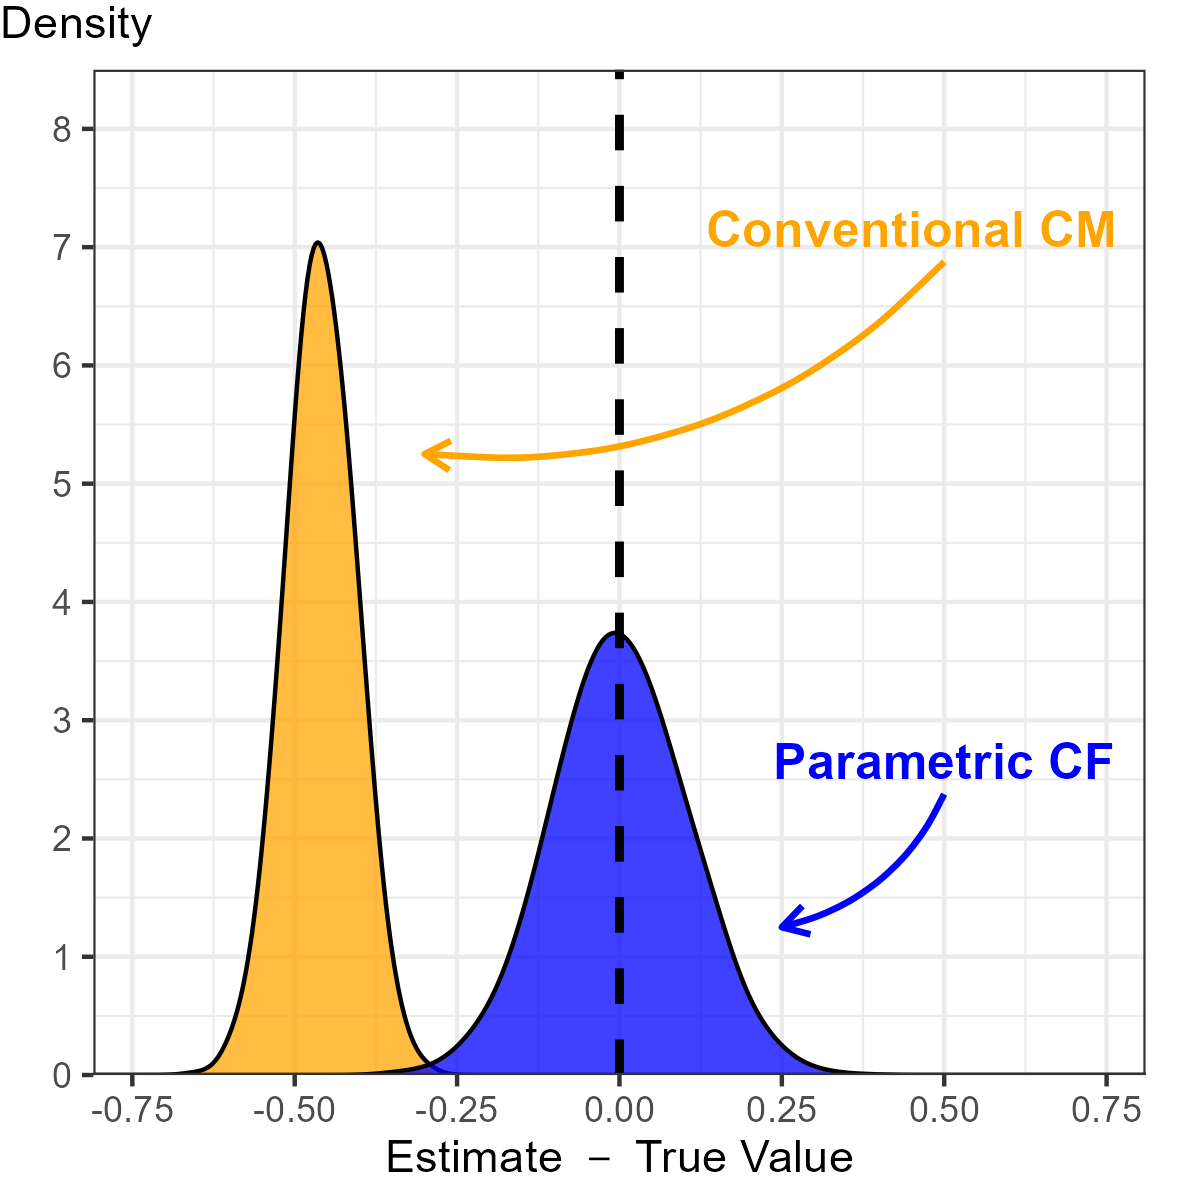
\includegraphics[width=\textwidth]{
                    ../text/sections/figures/normal-direct-dist.png}
            \end{subfigure}
            \begin{subfigure}[c]{0.525\textwidth}
                \centering
                \caption{$\hat{\text{AIE}} - \text{AIE}$.}
                \vskip-0.25cm
                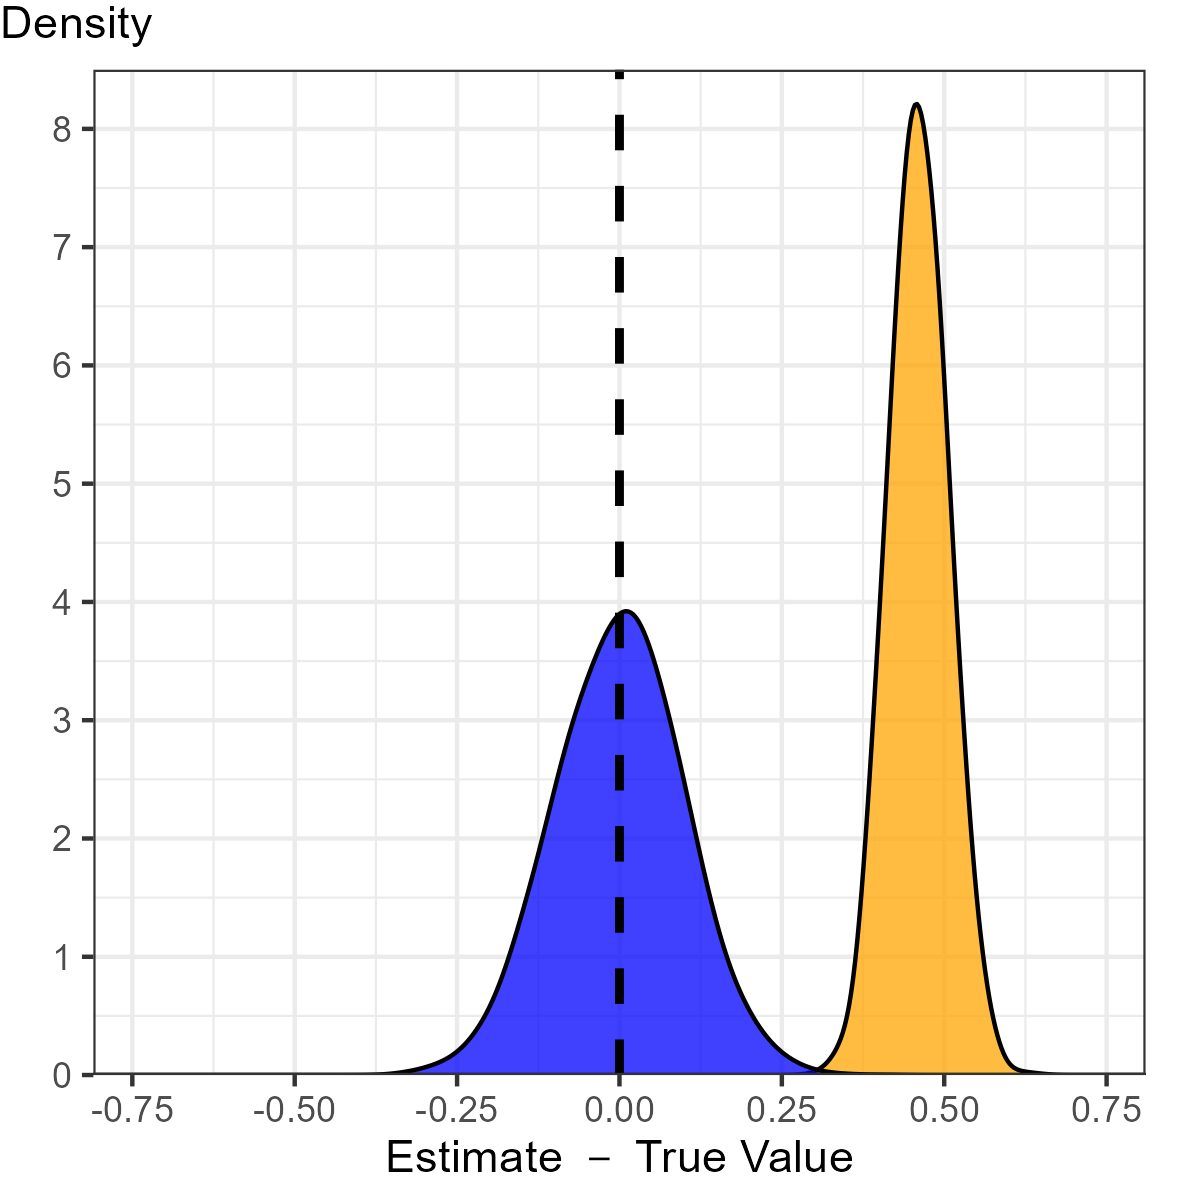
\includegraphics[width=\textwidth]{
                    ../text/sections/figures/normal-indirect-dist.png}
            \end{subfigure}
        \end{figure}
    }}
\end{frame}

%-------------------------------------------------------------------------------
\begin{frame}
    \frametitle{2. CM with Selection --- Estimation}
    In practice, this means two-stage CM estimation, with CF in second-stage.

    \par\noindent\rule{\textwidth}{0.4pt}
    \textbf{Parametric CF Estimation Recipe:}
    \begin{enumerate}
        \item Estimate mediation first-stage with probit, including the IV.
        \item Estimate mediation second-stage by OLS, with Mills ratio CF terms (Heckman 1979).
        \item Compose CM estimates from two-stage plug-in estimates
        \\(same as parametric MTEs, Bj{\"o}rklund Moffitt 1987).
    \end{enumerate}

    \vskip0.5cm
    \onslide<2->{
        \textbf{Semi-parametric CF Estimation Recipe:} \\
        Replace \textbf{2.} with semi-parametric CFs
        (same estimation as MTEs).}

    \vfill
    \onslide<1->{
    \par\noindent\rule{\textwidth}{0.4pt}
    $\implies$ Conventional CM estimates (two-stages) $+$ IV-guided CF adjustment.}
\end{frame}
%-------------------------------------------------------------------------------
\begin{frame}
    \frametitle{2. CM with Selection --- Estimation}
    \vskip-0.25cm
    \makebox[\textwidth]{\parbox{1.25\textwidth}{
        \begin{figure}
            \caption{CM Estimates from 10,000 DGPs with \textbf{Uniform} Errors.}
            \vskip-0.25cm
            \begin{subfigure}[c]{0.525\textwidth}
                \centering
                \caption{$\hat{\text{ADE}} - \text{ADE}$.}
                \vskip-0.25cm
                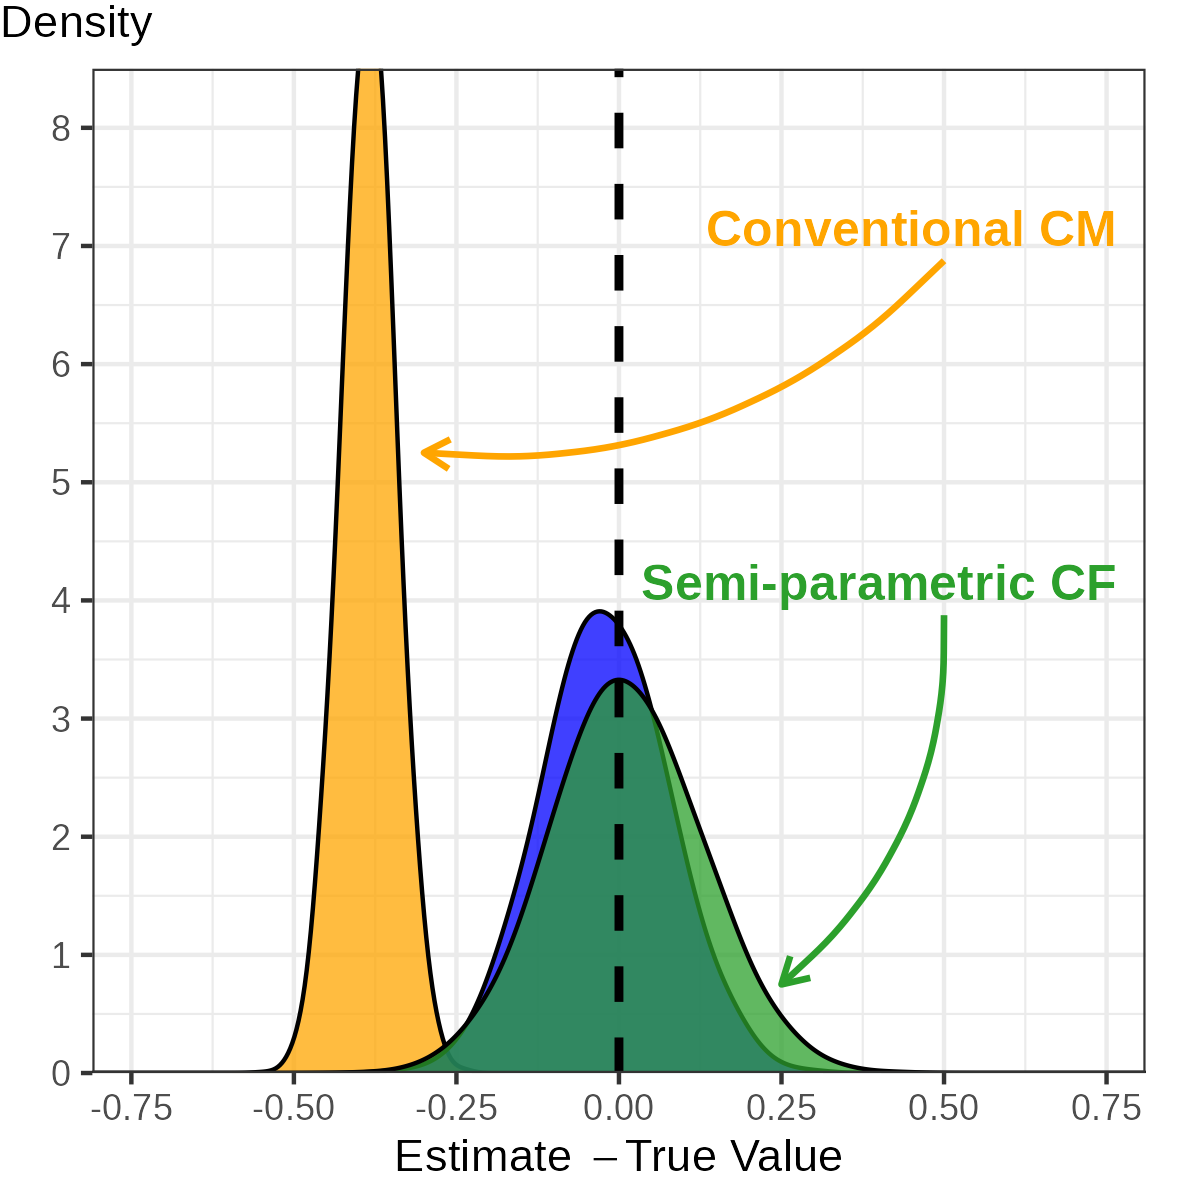
\includegraphics[width=\textwidth]{
                    ../text/sections/figures/uniform-direct-dist.png}
                    %../programs/simulations/sim-output/uniform-direct-dist.png}
            \end{subfigure}
            \begin{subfigure}[c]{0.525\textwidth}
                \centering
                \caption{$\hat{\text{AIE}} - \text{AIE}$.}
                \vskip-0.25cm
                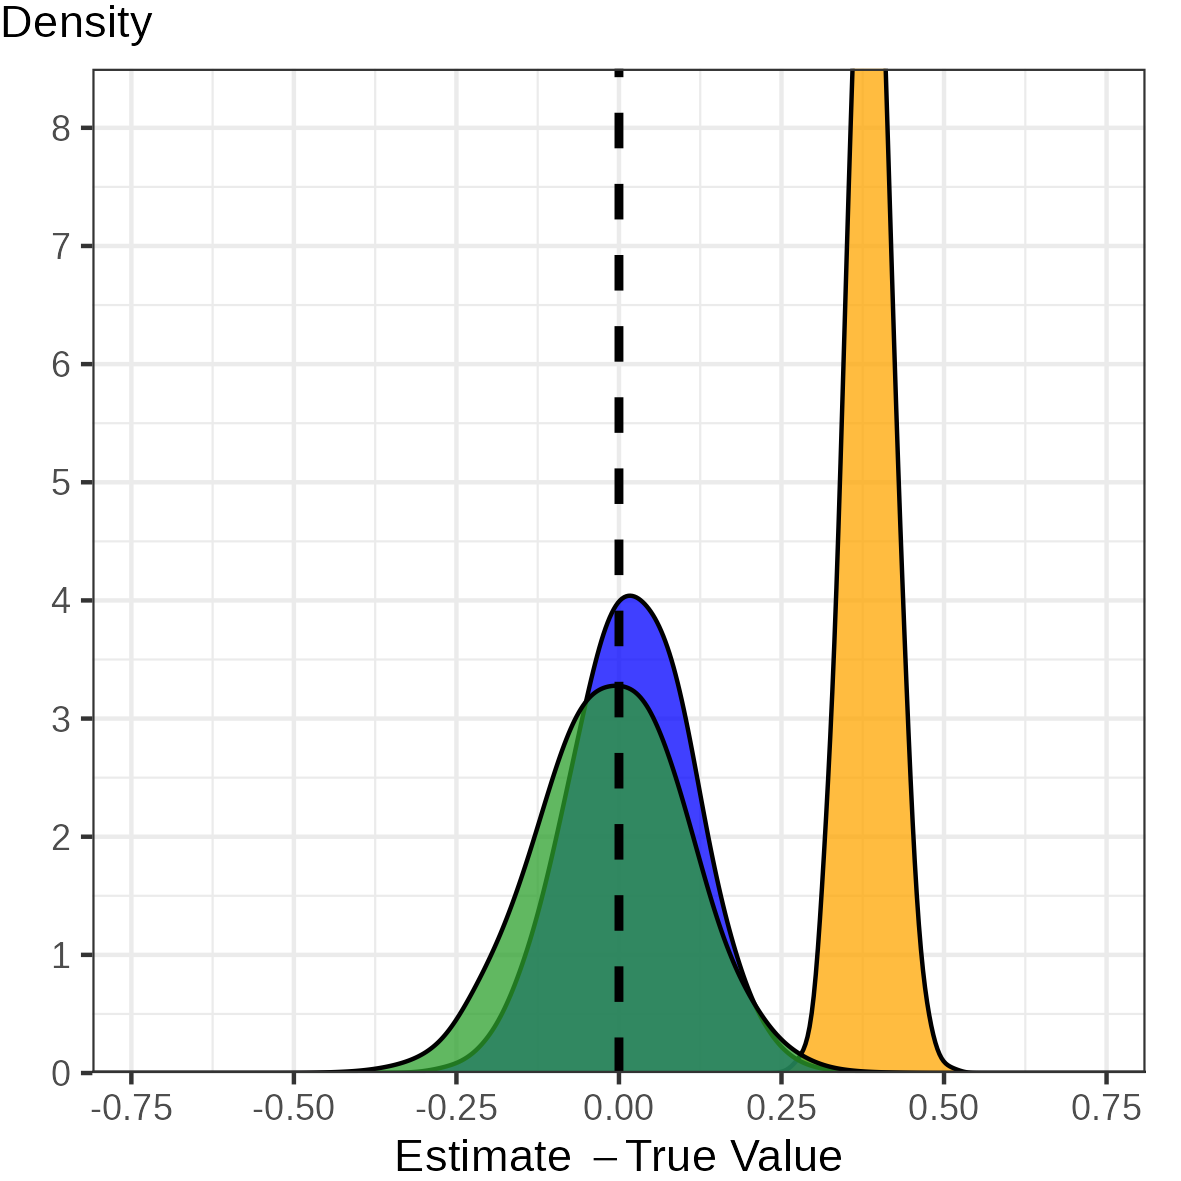
\includegraphics[width=\textwidth]{
                    ../text/sections/figures/uniform-indirect-dist.png}
                    %../programs/simulations/sim-output/uniform-indirect-dist.png}
            \end{subfigure}
        \end{figure}
    }}
\end{frame}
%-------------------------------------------------------------------------------
\section{3. Oregon}
%-------------------------------------------------------------------------------
\begin{frame}
    \frametitle{3. Returning to Oregon}
    Winning access to Medicaid increases healthcare usage, and subjective health:
    \vskip-0.375cm
    \begin{figure}
        %\caption{Oregon Health Insurance Experiment (OHIE) Suggestive Mechanism.}
        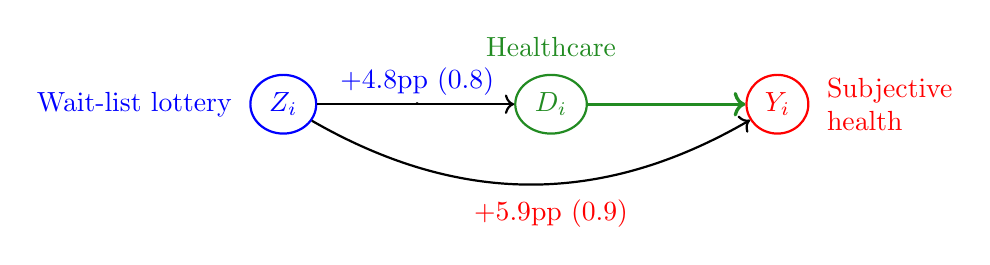
\begin{tikzpicture}
            \node[state,thick,ForestGreen] (mediator) at (0,0) {$D_i$};
            \node[state,thick,blue] (treatment) [left=2.5cm of mediator] {$Z_i$};
            \node[state,thick,red] (outcome)   [right=2cm of mediator] {$Y_i$};
            % Label Z_i, D, Y_i
            \node[color=ForestGreen] [above=0.1cm of mediator] {Healthcare};
            \node[color=blue] [left=0.1cm of treatment] {Wait-list lottery};
            \node[color=red,align=left] [right=0.1cm of outcome] {Subjective \\ health};
            % Draw the causal arrows
            \path[->, thick] (treatment) edge (mediator);
            \path[->, thick] (treatment) edge[bend right=30] (outcome);
            % Label the effect sizes.
            \node[color=black] (firststage) at ($(mediator)!0.5!(treatment)$) {.};
            \node[color=blue] [above=-0.15cm of firststage] {+4.8pp (0.8)};
            \node[color=red] [below=0.7cm of mediator] {+5.9pp (0.9)};
            \pause
            \path[->, very thick, color=ForestGreen] (mediator) edge (outcome);
        \end{tikzpicture}
    \end{figure}
    \vskip-0.25cm

    \par\noindent\rule{\textwidth}{0.4pt}
    \pause
    \textbf{CM} is quantitatively estimating the entire system:
    \begin{itemize}
        \item Use correlational estimate of $\textcolor{ForestGreen}{D_i} \to \textcolor{red}{Y_i}$
        \item Does \textcolor{ForestGreen}{visiting healthcare} at least once increase \textcolor{red}{subjective health} 12 months later?
        \item OLS for $\textcolor{ForestGreen}{D_i} \to \textcolor{red}{Y_i}$ is \textcolor{ForestGreen}{$\approx 0$} (not significant).
    \end{itemize}
\end{frame}
%-------------------------------------------------------------------------------
\begin{frame}
    \frametitle{3. Returning to Oregon}
    Conventional CM estimates lottery effects as mostly direct, $\approx 0$ healthcare.
    \vskip0.5cm
    
    \begin{figure}
        %\caption{CM Estimates in the Oregon Health Insurance Experiment.}
        %\vskip-0.25cm
        \centering
        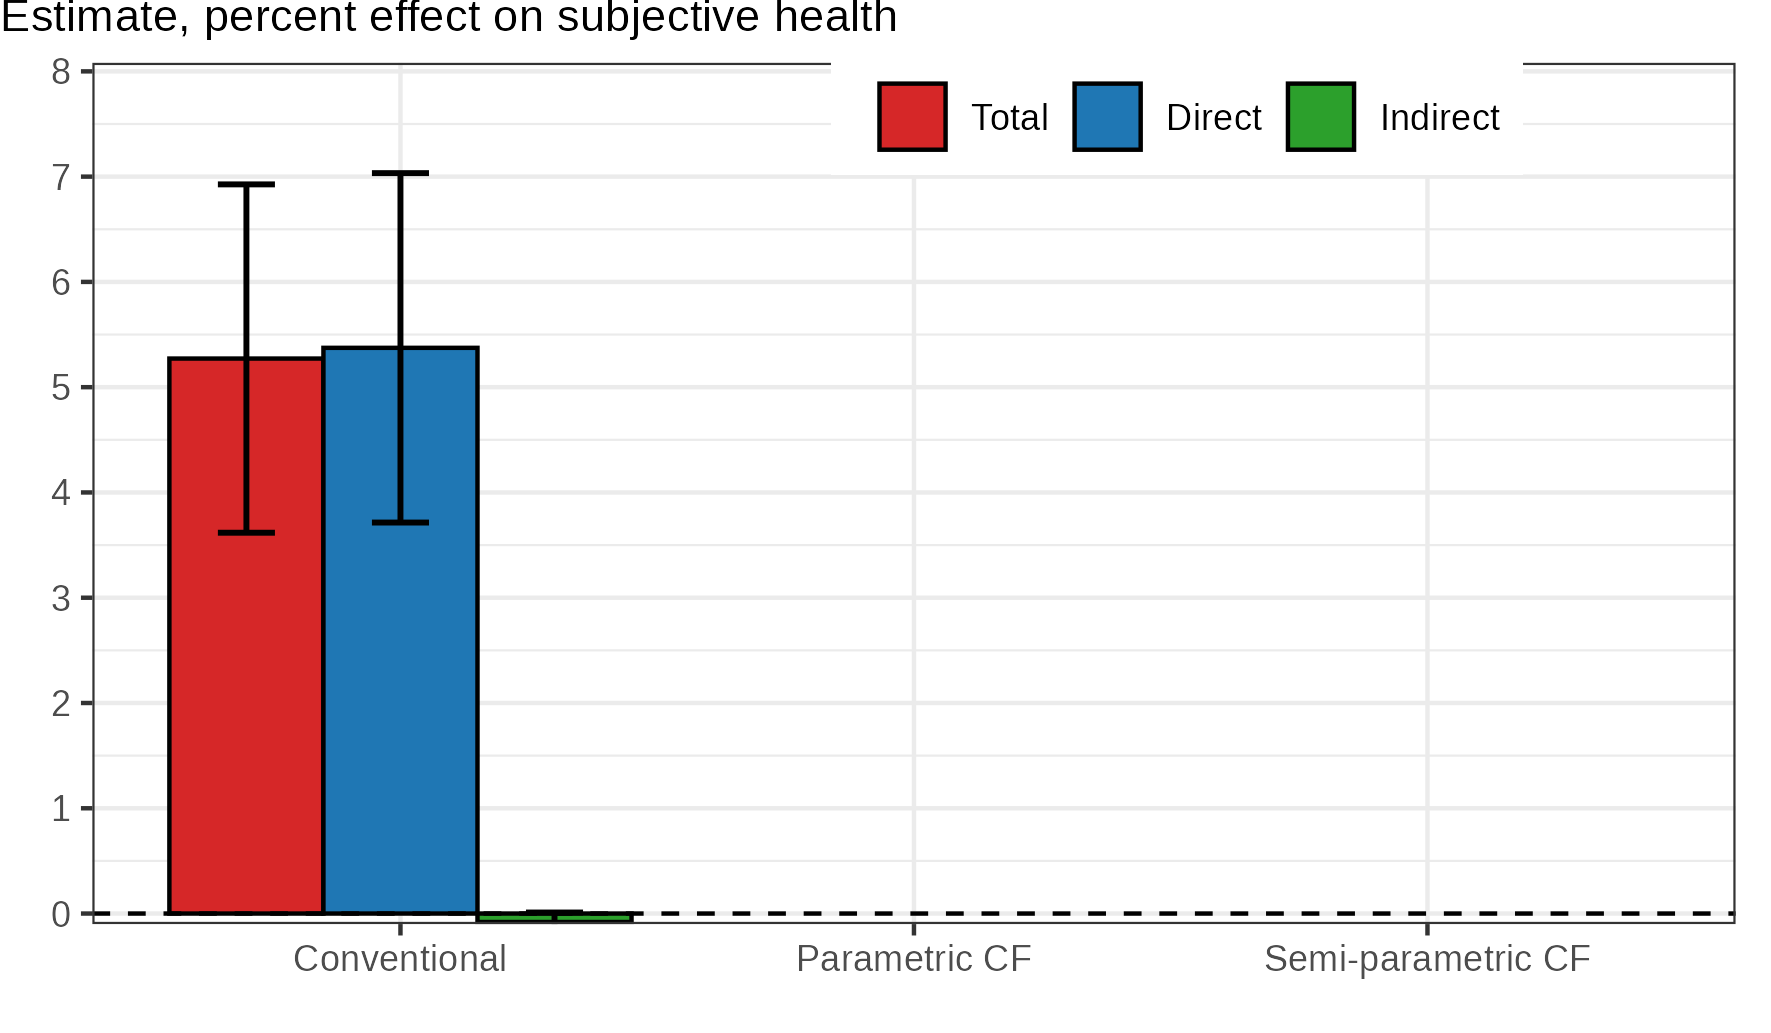
\includegraphics[width=0.9\textwidth]{
            ../text/sections/figures/mediation-health-placeholder.png}
    \end{figure}

\end{frame}
%-------------------------------------------------------------------------------
\begin{frame}
    \frametitle{3. Returning to Oregon}
    Winning access to Medicaid increases healthcare usage, and subjective health:
    \vskip-0.375cm
    \begin{figure}
        %\caption{Oregon Health Insurance Experiment (OHIE) Suggestive Mechanism.}
        
\begin{tikzpicture}
            \node[state,thick,ForestGreen] (mediator) at (0,0) {$D_i$};
            \node[state,thick,blue] (treatment) [left=2cm of mediator] {$Z_i$};
            \node[state,thick,red] (outcome)   [right=2.5cm of mediator] {$Y_i$};
            % Label Z_i, D, Y_i
            \node[color=ForestGreen] [above=0.1cm of mediator] {Healthcare};
            \node[color=blue] [left=0.1cm of treatment] {Wait-list lottery};
            \node[color=red,align=left] [right=0.1cm of outcome] {Subjective \\ health};
            % Draw the causal arrows
            \path[->, thick] (treatment) edge (mediator);
            \path[->, thick] (treatment) edge[bend right=30] (outcome);
            % Label the effect sizes.
            \pause
            \path[->, very thick, color=orange] (mediator) edge (outcome);
            \node[color=orange] (aie) at ($(mediator)!0.5!(outcome)$) {.};
            \node[color=orange] [above=-0.15cm of aie] {Complier};
            \node[color=orange] [below=-0.15cm of aie] {indirect};
        \end{tikzpicture}
    \end{figure}
    \vskip-0.25cm

    \par\noindent\rule{\textwidth}{0.4pt}
    \pause
    My approach to \textbf{CM} is modelling selection-into-$\textcolor{ForestGreen}{D_i}$ via \textcolor{orange}{mediator MTE}:
    \begin{itemize}
        \item Uses an estimate of $\textcolor{ForestGreen}{D_i} \to \textcolor{red}{Y_i}$ (plus complier extrapolation)
        \item Regular healthcare location pre-lottery serves as first-stage IV \hyperlink{ohie-iv}{\beamergotobutton{IV}}.
        \item IV $+$ CF extrapolation estimates of $\textcolor{ForestGreen}{D_i} \to \textcolor{red}{Y_i}$ are larger \\$\implies$ smaller ADE estimates.
    \end{itemize}
\end{frame}
%-------------------------------------------------------------------------------
\begin{frame}
    \frametitle{3. Returning to Oregon}
    Using my approach, with regular healthcare location as an excluded IV, restores indirect effect through increasing healthcare visitation.
    \vskip0.5cm
    
    \begin{figure}
        %\caption{CM Estimates in the Oregon Health Insurance Experiment.}
        %\vskip-0.25cm
        \centering
        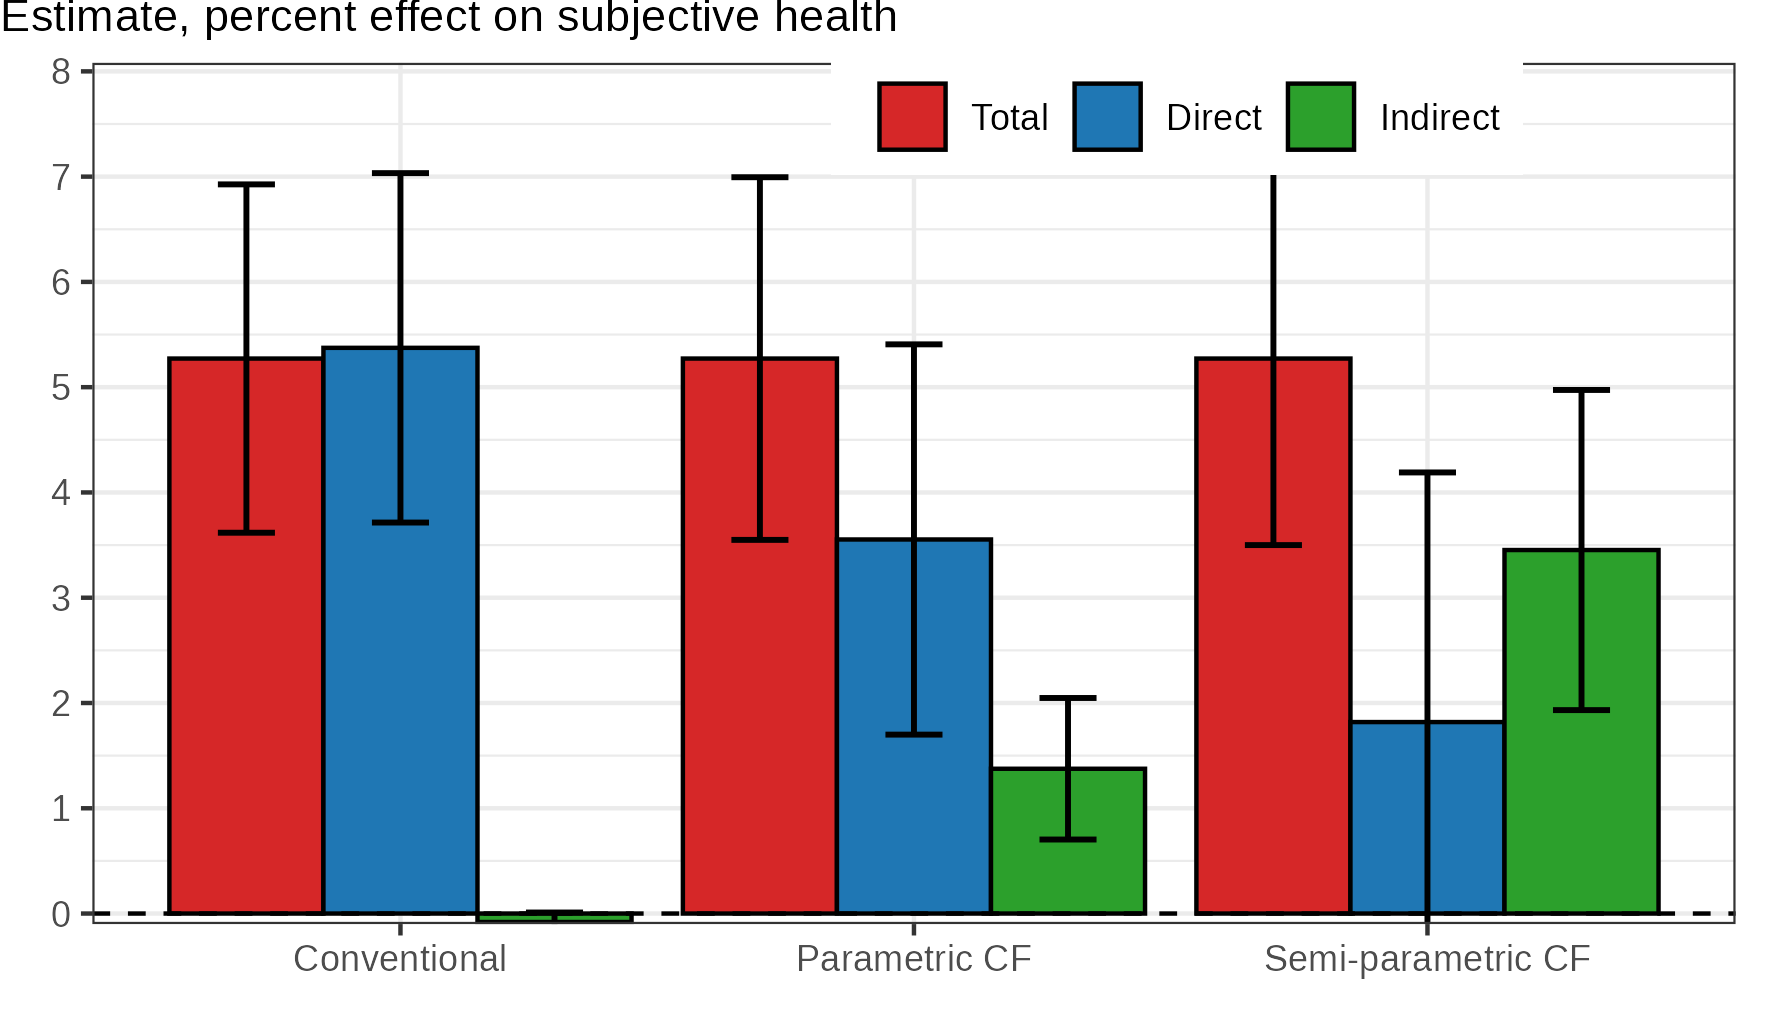
\includegraphics[width=0.9\textwidth]{
            ../text/sections/figures/mediation-health.png}
    \end{figure}
\end{frame}
%-------------------------------------------------------------------------------
\section{Conclusion}
%-------------------------------------------------------------------------------
\begin{frame}
    \frametitle{Conclusion}
    \textbf{Overview:}
    \begin{enumerate}
        \item CM as alternative to ``suggestive evidence for mechanisms.''
        \item Selection bias in conventional CM analyses with no case for mediator ignorability.
        \item Connect CM with labour theory $+$ selection-into-treatment $+$ MTEs.
    \end{enumerate}
    \par\noindent\rule{\textwidth}{0.4pt}

    \textbf{Caveats and points to remember:}
    \begin{itemize}
        \item Structural assumptions and IV for identification $+$ estimation (not ideal).
        \item Application to Oregon Health Insurance Experiment, showing subjective health $+$ well-being effects mediated by healthcare.
        \item \hl{\textbf{Credible} analyses of mechanisms are hard in practice, wide confidence intervals show true uncertainty.}
    \end{itemize}
\end{frame}
%-------------------------------------------------------------------------------
\section{Appendix}
%-------------------------------------------------------------------------------
\begin{frame}[noframenumbering]
    \frametitle{Appendix: CM Guiding Model}
    \label{cm-model}
    Consider binary \textcolor{blue}{treatment $Z_i = 0, 1$},
    binary \textcolor{ForestGreen}{mediator $D_i = 0, 1$},
    and continuous \textcolor{red}{outcome $Y_i$}.
    \vskip-1.25cm
    \begin{figure}
        \centering
        \singlespacing
        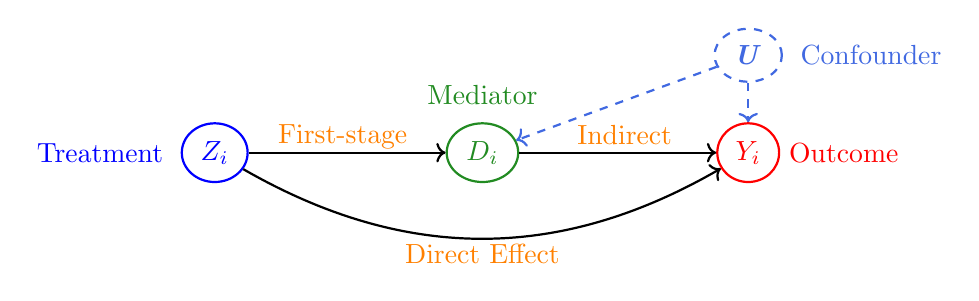
\begin{tikzpicture}
            \node[state, thick,ForestGreen] (mediator) at (0,0) {$D_i$};
            \node[state, thick,blue] (treatment) [left=2.5cm of mediator] {$Z_i$};
            \node[state, thick,red] (outcome) [right=2.5cm of mediator] {$Y_i$};
            % Label Z, D, Y
            \node[color=ForestGreen] [above=0.1cm of mediator] {Mediator};
            \node[color=blue] [left=0.1cm of treatment] {Treatment};
            \node[text width=0.1cm, color=red] [right=-0.01cm of outcome] {Outcome};
            % Draw the causal arrows
            \path[->, thick] (treatment) edge (mediator);
            \path[->, thick] (mediator) edge (outcome);
            \path[->, thick] (treatment) edge[bend right=30] (outcome);
            % Label direct and indirect effect
            \node[color=orange] [above left=-0.35cm and 0.5cm of mediator] {First-stage};
            \node[color=orange] [above right=-0.3cm and 0.75cm of mediator] {Indirect};
            \node[color=orange] [below=0.65cm of mediator] {Direct Effect};
            % Add in the confounders
            %\node[state, thick,RoyalPurple] (confounderX) [above=1.5cm of mediator] {$\vec{X}$};
            %\path[->,RoyalPurple] (confounderX) edge (mediator);
            %\node[color=RoyalPurple] [left=0.1cm of confounderX] {Observed controls};
            \node[state, thick,dashed,thick,RoyalBlue] (confounderU) [
                above=0.5cm of outcome] {$\vec U$};
            \node[color=RoyalBlue] [right=0.1cm of confounderU] {Confounder};
            \path[->,thick,dashed,color=RoyalBlue] (confounderU) edge (mediator);
            \path[->,thick,dashed,color=RoyalBlue] (confounderU) edge (outcome);
            %\node[color=RoyalBlue] [right=0.1cm of confounderU] {Unobserved confounder};
        \end{tikzpicture}
    \end{figure}
    \vskip-0.5cm
    \par\noindent\rule{\textwidth}{0.4pt}
    \[ \text{Average Direct Effect (ADE)}: \;\;\;
        \E{Y_i\left(\eqhighlight{blue}{1}, D_i(Z_i) \right)
            - Y_i\left(\eqhighlight{blue}{0}, D_i(Z_i) \right)} \]
    \vskip-0.35cm
    \begin{itemize}
        \item ADE is causal effect $Z\to Y$, blocking the indirect $D_i$ path.
    \end{itemize}
    \vskip0.25cm
    \[ \text{Average Indirect Effect (AIE):} \;\;\;
    \E{Y_i\left(Z_i, \eqhighlight{ForestGreen}{D_i(1)} \right)
        - Y_i\left(Z_i, \eqhighlight{ForestGreen}{D_i(0)} \right)} \]
    \vskip-0.25cm
    \begin{itemize}
        \item AIE is causal effect of $D_i(Z_i) \to Y_i$, blocking the direct $Z_i$ path.
    \end{itemize}
\end{frame}
%-------------------------------------------------------------------------------
\begin{frame}[noframenumbering]
    \frametitle{Group Difference --- ADE}
    \label{group-diff-ade}
    CM effects contaminated by (less interpretable) bias terms.
    \[ \text{\textcolor{purple}{CM Estimand}}
        = \text{\textcolor{blue}{ADEM}}
            + \text{\textcolor{red}{Selection Bias}} \]
    \vspace{-0.25cm}
    {\footnotesize
    \begin{align*}
        & \underbrace{\mathbb E_{D_i} \Big[
            \Egiven{Y_i}{Z_i = 1, D_i} - \Egiven{Y_i}{Z_i = 0, D_i} \Big]}_{
                \text{\textcolor{purple}{Estimand, Direct Effect}} } \\
        & = \underbrace{\E[D_i= d']{
            \Egiven{Y_i(1, D_i(Z_i)) - Y_i(0, D_i(Z_i))}{D_i(1) = d'}} }_{
            \text{\textcolor{blue}{Average Direct Effect on Mediator (ADEM) take-up --- i.e., $D_i(1)$ weighted}}} \\
        & \;\;\;\; + \underbrace{ \mathbb E_{D_i} \Big[ 
            \Egiven{Y_i(0, D_i(Z_i))}{D_i(1) = d'} 
            - \Egiven{Y_i(0, D_i(Z_i))}{D_i(0) = d'} \Big] }_{
                \text{\textcolor{red}{Selection Bias}}}
    \end{align*}}
    The weighted ADE you get here is a positive weighted sum of local ADEs, but with policy irrelevant weights $D_i(1) = d'$.

    \vskip0.5cm
    $\implies$ consider this group bias, noting difference from true ADE.
    \hyperlink{main:selection-bias}{\beamergotobutton{Back}}
\end{frame}
%-------------------------------------------------------------------------------
\begin{frame}[noframenumbering]
    \frametitle{Selection Bias --- Direct Effect}
    CM Effects $+$ contaminating bias.
    \[ \text{\textcolor{purple}{CM Estimand}}
        = \text{\textcolor{blue}{ADE}}
            + \Big(\text{\textcolor{red}{Selection Bias}}
            + \text{\textcolor{orange}{Group difference bias}}\Big) \]
    \hyperlink{cm-model}{\beamergotobutton{Model}}
    \vskip-0.25cm

    \par\noindent\rule{\textwidth}{0.4pt}
    {\footnotesize
    \begin{align*}
        & \underbrace{\mathbb E_{D_i=d'} \Big[
            \Egiven{Y_i}{Z_i = 1, D_i=d'} - \Egiven{Y_i}{Z_i = 0, D_i=d'} \Big]}_{
                \text{\textcolor{purple}{Estimand, Direct Effect}} } \\
        & = \underbrace{\E{Y_i(1, D_i(Z_i)) - Y_i(0, D_i(Z_i))}}_{
            \text{\textcolor{blue}{Average Direct Effect}}} \\
        & \;\;\;\; + 
        \underbrace{ \mathbb E_{D_i=d'} \Big[ 
            \Egiven{Y_i(0, D_i(Z_i))}{D_i(1) = d'} 
            - \Egiven{Y_i(0, D_i(Z_i))}{D_i(0) = d'} \Big] }_{
                \text{\textcolor{red}{Selection Bias}}} \\
        & \;\;\;\; + \underbrace{ \E[D_i =d']{
            \begin{aligned}
            &\Big(1 - \Prob{D_i(1) = d'} \Big) \\
            &\times \left( \begin{aligned}
                &\Egiven{Y_i(1, D_i(Z_i)) - Y_i(0, D_i(Z_i))}{D_i(1) = 1-d'} \\ 
                &  - \Egiven{Y_i(1, D_i(Z_i)) - Y_i(0, D_i(Z_i))}{D_i(0) = d'}
                \end{aligned} \right) \end{aligned}} }_{
                    \text{\textcolor{orange}{Group difference bias} 
                        \hyperlink{group-diff-ade}{\beamergotobutton{Group-diff}}}}
    \end{align*}}
\end{frame}
%-------------------------------------------------------------------------------
\begin{frame}[noframenumbering]
    \frametitle{Group Difference --- AIE}
    \label{group-diff-aie}
    CM effects contaminated by (less interpretable) bias terms.
    \[ \text{\textcolor{purple}{CM Estimand}}
        = \text{\textcolor{ForestGreen}{AIEM}}
            + \Big(\text{\textcolor{red}{Selection Bias}}
            + \text{\textcolor{orange}{Group difference bias}}\Big) \]
    \vspace{-0.25cm}
    {\footnotesize
    \begin{align*}
        & \underbrace{\E[Z_i]{
            \Big( \Egiven{D_i}{Z_i = 1} - \Egiven{D_i}{Z_i = 0} \Big) \times
            \Big( \Egiven{Y_i}{Z_i, D_i = 1} - \Egiven{Y_i}{Z_i, D_i = 0} \Big) }}_{ \text{\textcolor{purple}{Estimand, Indirect Effect}} } \\
        & = \underbrace{
                \Egiven{Y_i(Z_i, D_i(1)) - Y_i(Z_i, D_i(0))}{D_i = 1}
            }_{\text{\textcolor{ForestGreen}{Average Indirect Effect on Mediated (AIEM) --- i.e., $D_i=1$ weighted}} } \\
        & \;\;\;\; + \underbrace{\bar \pi  \Big(
            \Egiven{Y_i(Z_i, 0)}{D_i = 1} - \Egiven{Y_i(Z_i, 0)}{D_i = 0} \Big)}_{
                \text{\textcolor{red}{Selection Bias}}} \\
        & \;\;\;\; + \underbrace{\bar \pi \left[
            \left( \frac{1 - \Prob{D_i(1) = 1, D_i(0) = 0} }{
                \Prob{D_i(1) = 1, D_i(0) = 0}} \right)
            \left( \begin{aligned}
                &\Egiven{Y_i(Z_i, 1) - Y_i(Z_i, 0)}{D_i(1) = 0 \text{ or } D_i(0)=1} \\ 
                &  - \E{Y_i(Z_i, 1) - Y_i(Z_i, 0)}
            \end{aligned} \right)
        \right]}_{\text{\textcolor{orange}{Groups difference Bias}}}
    \end{align*}}
    The weighted AIE you get here is not a positive weighted sum of local AIEs, 
    because the AIE is only about $D(Z)$ compliers.
    \hyperlink{cm-model}{\beamergotobutton{Model}}.

    $\implies$ consider this group bias, noting difference from true AIE.
    \hyperlink{main:selection-bias}{\beamergotobutton{Back}}
\end{frame}
%-------------------------------------------------------------------------------
\begin{frame}[noframenumbering]
    \frametitle{Selection Bias --- Indirect Effect}
    CM Effects $+$ contaminating bias, where $\bar\pi = \Prob{D_i(0) \neq D_i(1)}$.
    \[ \text{\textcolor{purple}{CM Estimand}}
        = \text{\textcolor{ForestGreen}{AIE}}
            + \Big(\text{\textcolor{red}{Selection Bias}}
            + \text{\textcolor{orange}{Group difference bias}}\Big) \hyperlink{cm-model}{\beamergotobutton{Model}} \]
    \vspace{-0.5cm}

    \par\noindent\rule{\textwidth}{0.4pt}
    {\footnotesize
    \begin{align*}
        & \underbrace{\E[Z_i]{
            \Big( \Egiven{D_i}{Z_i = 1} - \Egiven{D_i}{Z_i = 0} \Big) \times
            \Big( \Egiven{Y_i}{Z_i, D_i = 1} - \Egiven{Y_i}{Z_i, D_i = 0} \Big) }}_{ \text{\textcolor{purple}{Estimand, Indirect Effect}} } \\
        & = \underbrace{\E{Y_i(Z_i, D_i(1)) - Y_i(Z_i, D_i(0))}}_{
            \text{\textcolor{ForestGreen}{Average Indirect Effect}} } \\
        & \;\;\;\; + \underbrace{\bar \pi  \Big(
            \Egiven{Y_i(Z_i, 0)}{D_i = 1} - \Egiven{Y_i(Z_i, 0)}{D_i = 0} \Big)}_{
                \text{\textcolor{red}{Selection Bias}}}\\
        & \;\;\;\; + \underbrace{ \bar\pi \left[ \begin{aligned}
            &\Big( 1 - \Prob{D_i=1} \Big)
            \left( \begin{aligned}
                &\Egiven{Y_i(Z_i, 1) - Y_i(Z_i, 0)}{D_i = 1} \\ 
                &  - \Egiven{Y_i(Z_i, 1) - Y_i(Z_i, 0)}{D_i = 0}
            \end{aligned} \right) \\
            &+ \left( \frac{1 - \Prob{D_i(1) = 1, D_i(0) = 0} }{
                \Prob{D_i(1) = 1, D_i(0) = 0}} \right)
            \left( \begin{aligned}
                &\Egiven{Y_i(Z_i, 1) - Y_i(Z_i, 0)}{D_i(Z_i) \neq Z_i} \\ 
                &  - \E{Y_i(Z_i, 1) - Y_i(Z_i, 0)}
            \end{aligned} \right)
        \end{aligned} \right]}_{\text{\textcolor{orange}{
            Groups difference Bias}
                \hyperlink{group-diff-aie}{\beamergotobutton{Group-diff}}}}
    \end{align*}}
\end{frame}
%-------------------------------------------------------------------------------
\begin{frame}[noframenumbering]
    \frametitle{Semi-parametric Control Functions}
    \label{cf-semiparametric}
    Semi-parametric specifications for the CFs $\lambda_0, \lambda_1$ bring some complications to estimating the AIE.
    \begin{align*}
        \Egiven{Y_i}{Z_i, D_i = 0, \vec X_i} &=
            \alpha + \gamma Z_i + \varphi\big( \vec X_i \big)
            + \eqhighlight{yellow}{\rho_0 \lambda_0 \big( \pi(Z_i ; \vec X_i) \big)}, \\
        \Egiven{Y_i}{Z_i, D_i = 1, \vec X_i} &=
            (\alpha + \beta) + (\gamma + \delta) Z_i + \varphi\big( \vec X_i\big)
            + \eqhighlight{yellow}{\rho_1 \lambda_1 \big( \pi(Z_i ; \vec X_i) \big)}.
    \end{align*}
    Intercepts, $\alpha, (\alpha + \beta)$, and relevance parameters $\rho_0, \rho_1$ are not separately identified from the CFs $\lambda_0(.), \lambda_1(.)$ so CF extrapolation term\\ $(\rho_1 - \rho_0) \Gamma \big(\pi(0; \vec X_i), \, \pi(1; \vec X_i) \big)$ is not directly identified or estimable.

    \par\noindent\rule{\textwidth}{0.4pt}    
    These problems can be avoided by estimating the AIE using its relation to the ATE, $\hat{\text{AIE}}^{\text{CF}} =$
    \[ \hat{\text{ATE}}
        - (1 - \bar Z) \, \underbrace{\left( 
            \frac 1N \sum_{i = 1}^N \hat\gamma + \hat \delta \, \hat\pi(1; \vec X_i) \right)}_{\hat{\text{ADE}}\text{ given }Z_i = 1}
        - \bar Z \, \underbrace{\left(
            \frac 1N \sum_{i = 1}^N \hat\gamma + \hat \delta \, \hat\pi(0; \vec X_i)  \right)}_{\hat{\text{ADE}}\text{ given }Z_i = 0}. \]
\end{frame}
%-------------------------------------------------------------------------------
\begin{frame}[noframenumbering]
    \frametitle{Appenidx: CM with Selection}
    Suppose $Z_i$ is ignorable, $D_i$ is not, so we have the following causal model.
    \vskip-0.75cm
    \begin{figure}
        \centering
        \singlespacing
        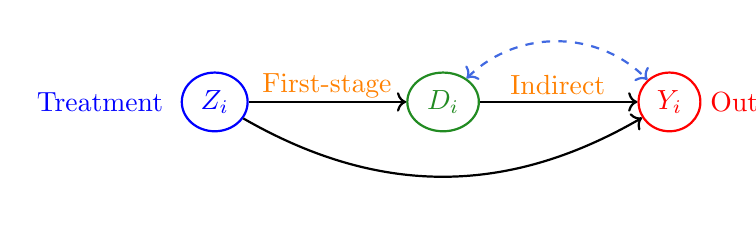
\begin{tikzpicture}
            \node[state, thick,ForestGreen] (mediator) at (0,0) {$D_i$};
            \node[state, thick,blue] (treatment) [left=2cm of mediator] {$Z_i$};
            \node[state, thick,red] (outcome) [right=2cm of mediator] {$Y_i$};
            % Label Z, D, Y
            %\node[color=ForestGreen] [above=0.1cm of mediator] {Mediator};
            \node[color=blue] [left=0.1cm of treatment] {Treatment};
            \node[text width=0.1cm, color=red] [right=-0.01cm of outcome] {Outcome};
            % Draw the causal arrows
            \path[->, thick] (treatment) edge (mediator);
            \path[->, thick] (mediator) edge (outcome);
            \path[->, thick] (treatment) edge[bend right=30] (outcome);
            % Label direct and indirect effect
            \node[color=orange] [above left=-0.35cm and 0.2cm of mediator] {First-stage};
            \node[color=orange] [above right=-0.3cm and 0.4cm of mediator] {Indirect};
            %\node[color=orange] [below=0.5cm of mediator] {Direct Effect};
            % Add in the unobserved confounding
            \path[<->,dashed,thick,color=RoyalBlue] (mediator) edge[bend right=-45] (outcome);
        \end{tikzpicture}
    \end{figure}
    \vskip-0.5cm
    
    \par\noindent\rule{\textwidth}{0.4pt}
    Then this system has the following random coefficient equations:
    \begin{align*}
        D_i &= \phi + \bar\pi Z_i + \varphi(\vec X_i) + U_i  \\
        Y_i &= \alpha + \beta D_i + \gamma Z_i + \delta Z_i D_i
        + \zeta(\vec X_i)
        + \underbrace{\eqhighlight{yellow}{
            \left(1 - D_i \right)U_{0,i} + D_i U_{1,i}}}_{
            \text{Correlated error term}}
    \end{align*}
    \vskip-0.5cm
    where $\beta, \gamma, \delta$ are functions of $\mu_{d'}(z'; \vec X_i)$.

    \par\noindent\rule{\textwidth}{0.4pt}
    \[ \text{ADE} = \E{\gamma + \delta D_i}, \;\;\;\;
    \text{AIE} = \E{ \bar \pi \big( \beta +  \delta Z_i + \tilde U_i \big)} \]
    with $\tilde U_i = \Egiven{ U_{1,i} - U_{0,i}}{
        \vec X_i, D_i(0) \neq D_i(1)}$ unobserved complier gains.
\end{frame}
%-------------------------------------------------------------------------------
\begin{frame}[noframenumbering]
    \frametitle{Appenidx: CM with Selection}
    Suppose $Z_i$ is ignorable, $D_i$ is not, so we have the following causal model.
    \vskip-0.75cm
    \begin{figure}
        \centering
        \singlespacing
        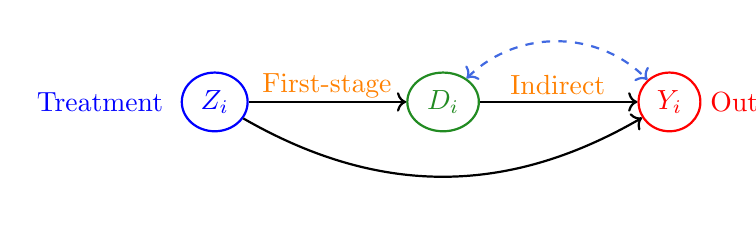
\begin{tikzpicture}
            \node[state, thick,ForestGreen] (mediator) at (0,0) {$D_i$};
            \node[state, thick,blue] (treatment) [left=2cm of mediator] {$Z_i$};
            \node[state, thick,red] (outcome) [right=2cm of mediator] {$Y_i$};
            % Label Z, D, Y
            %\node[color=ForestGreen] [above=0.1cm of mediator] {Mediator};
            \node[color=blue] [left=0.1cm of treatment] {Treatment};
            \node[text width=0.1cm, color=red] [right=-0.01cm of outcome] {Outcome};
            % Draw the causal arrows
            \path[->, thick] (treatment) edge (mediator);
            \path[->, thick] (mediator) edge (outcome);
            \path[->, thick] (treatment) edge[bend right=30] (outcome);
            % Label direct and indirect effect
            \node[color=orange] [above left=-0.35cm and 0.2cm of mediator] {First-stage};
            \node[color=orange] [above right=-0.3cm and 0.4cm of mediator] {Indirect};
            %\node[color=orange] [below=0.5cm of mediator] {Direct Effect};
            % Add in the unobserved confounding
            \path[<->,dashed,thick,color=RoyalBlue] (mediator) edge[bend right=-45] (outcome);
        \end{tikzpicture}
    \end{figure}
    \vskip-0.5cm
    
    \par\noindent\rule{\textwidth}{0.4pt}
    Main problem, second-stage is not identified:
    \begin{align*}
        \Egiven{Y_i}{Z_i, D_i, \vec X_i} \;\; =& \;\;
            \alpha
            + \beta D_i
            + \gamma Z_i
            + \delta Z_i D_i
            + \varphi(\vec X_i) \\
            & \;\; + \eqhighlight{yellow}{
                \left( 1 - D_i \right) \Egiven{ U_{0,i} }{D_i = 0, \vec X_i}} \\
            & \;\; + \underbrace{\eqhighlight{yellow}{
                D_i \Egiven{ U_{1,i} }{D_i = 1, \vec X_i}}}_{
                    \text{Unobserved $D_i$ confounding.}}
    \end{align*}
    \vfill

    \par\noindent\rule{\textwidth}{0.4pt}
    \textbf{Identification intuition:}
    Identify second-stage via MTE control function.
\end{frame}
%-------------------------------------------------------------------------------
\begin{frame}[noframenumbering]
    \frametitle{Appenidx: CM with Selection --- Identification}
    Assume:
    \begin{enumerate}
        \item Mediator monotonicity,
        $\Probgiven{ D_i(0) \leq D_i(1) }{\vec X_i} = 1$
        \[ \implies D_i(z') = \indicator{U_i \leq \pi(z'; \vec X_i)},
            \;\;\; \text{for } z'=0,1 \text{  (Vycatil 2002)}. \]
        \item Selection on mediator benefits,
        $\Cov{U_i, \, U_{0,i}}, \; \Cov{U_i, \, U_{1,i}} \neq 0$
        \[ \implies \text{First-stage take-up informs second-stage confounding.} \]
        \item There is an IV for the mediator, $\vec X_i^{\text{IV}}$ among control variables $\vec X_i$.
        \[ \implies \pi(Z_i ; \vec X_i) = \Probgiven{D_i = 1}{Z_i,\vec X_i} 
        \text{ is separately identified.} \]
    \end{enumerate}
    \par\noindent\rule{\textwidth}{0.4pt}
    \textbf{Proposition:}

    \vskip-0.5cm
    \begin{align*}
        & \Egiven{Y_i(z', 1) - Y_i(z', 0)}{Z_i = z', \vec X_i, U_i = p'} \\
        &= \beta + \delta z' + \Egiven{U_{1,i} - U_{0,i}}{\vec X_i, U_i = p'},
        \;\;\;\; \text{ for } p' \in (0,1).
    \end{align*}
\end{frame}
%-------------------------------------------------------------------------------
\begin{frame}[noframenumbering]
    \frametitle{Appenidx: CM with Selection --- Identification}
    The marginal effect has corresponding Control Functions (CFs), describing unobserved selection-into-$D_i$,
    \[ \rho_0 \lambda_0(p') = \Egiven{ U_{0,i} }{ p' \leq U_i }, \;\;\;\;
        \rho_1 \lambda_1(p') = \Egiven{ U_{1,i} }{ U_i \leq p' }. \]

    \vskip-0.25cm
    \par\noindent\rule{\textwidth}{0.4pt}
    These CFs restore second-stage identification, by extrapolating from $\vec X_i^{\text{IV}}$ compliers to $D_i(Z_i)$ mediator compliers,
    \begin{align*}
        \Egiven{Y_i}{Z_i, D_i, \vec X_i} \;\; =& \;\;
            \alpha
            + \beta D_i
            + \gamma Z_i
            + \delta Z_i D_i
            + \varphi(\vec X_i) \\
            & \;\; + \underbrace{\eqhighlight{yellow}{
                \rho_0 \left( 1 - D_i \right) \lambda_0 \big( \pi(Z_i ; \vec X_i) \big)
                + \rho_1 D_i \lambda_1 \big( \pi(Z_i ; \vec X_i) \big)}}_{
                    \text{CF adjustment.}}
    \end{align*}

    \par\noindent\rule{\textwidth}{0.4pt}
    This adjusted second-stage re-identifies the ADE and AIE,
    
    \makebox[\textwidth]{\parbox{1.25\textwidth}{
        \small
        \[ \text{ADE}
            = \E{\gamma + \delta D_i},
        \text{ AIE}
            = \mathbb E \Bigg[ \, \bar \pi \,
                \Big( \beta +  \delta Z_i +
                    \underbrace{ (\rho_1 - \rho_0) \,
                    \Gamma \big(\pi(0; \vec X_i), \, \pi(1; \vec X_i) \big)}_{
                        \text{Mediator compliers extrapolation.}} \Big) \Bigg] \]
    }}
\end{frame}
%-------------------------------------------------------------------------------
\begin{frame}[noframenumbering]
    \frametitle{Appenidx: CM with Selection --- Estimation}
    Will explain how estimation works, with simulation evidence.
    \vskip0cm
    \begin{enumerate}
        \item $\text{\textcolor{blue}{Random treatment $Z_i$}}
            \sim \text{Binom}\left(0.5 \right)$, for $n = 5,000$.
        \item $ \eqhighlight{yellow}{
            \left( U_{0,i}, U_{1,i} \right) \sim
        \text{BivariateNormal}\left( 0, 0, \sigma_0, \sigma_1, \rho \right)},
            \;\; \text{Costs }C_i \sim N(0, 0.5). $
    \end{enumerate}
    \par\noindent\rule{\textwidth}{0.4pt}
    Roy \textcolor{ForestGreen}{selection-into-$D_i$}, with constant partial effects $+$ interaction term.
    \begin{align*}
        D_i(z')    &= \indicator{C_i \leq Y_i(z', 1) - Y_i(z', 0)},&  \\
        Y_i(z',d') &= \left( z' + d' + z' d' \right) + U_{d'}
        & \text{ for } z',d' = 0,1.
    \end{align*}
    \par\noindent\rule{\textwidth}{0.4pt}
    Following the previous, these data have the following first and second-stage equations, where $\vec X_i^\text{IV}$ is an additive cost IV:
    \begin{align*}
        D_i &= \indicator{
            C_i - \Big( \eqhighlight{yellow}{U_{1,i} - U_{0,i}} \Big)
                \leq Z_i - \vec X_i^{\text{IV}} } \\
        Y_i &= Z_i + D_i + Z_i D_i
            + \eqhighlight{yellow}{
                \left( 1 - D_i \right) U_{0,i} + D_i U_{1,i}}.
    \end{align*}
    \small
    $\implies$ unobserved confounding by BivariateNormal $\Big(U_{0,i}, U_{1,i}\Big)$.
\end{frame}
%-------------------------------------------------------------------------------
\begin{frame}[noframenumbering]
    \frametitle{Appenidx: CM with Selection --- Estimation}
    Errors are normal, so system is Heckman (1979) selection model.

    \vskip0.25cm

    CFs are the inverse Mills ratio, with $\phi(.)$ normal pdf and $\Phi(.)$ normal cdf, 
    \[ \lambda_0(p') =
        \frac{\phi( - \Phi^{-1}(p') )}{\Phi( -\Phi^{-1}(p') )}, \;\;\;\;
    \lambda_1(p') =
        \frac{\phi( \Phi^{-1}(p') )}{\Phi( \Phi^{-1}(p') )},
        \;\;\;\; \text{ for } p' \in (0,1). \]

    \par\noindent\rule{\textwidth}{0.4pt}
    \textbf{Parametric Estimation Recipe:}
    \begin{enumerate}
        \item Estimate first-stage $\pi(Z_i; \vec X_i)$ with probit, including $\vec X_i^{\text{IV}}$.
        \item \hl{Include $\lambda_0, \lambda_1$ CFs in second-stage} OLS estimation.
        \item Compose CM estimates from two-stage plug-in estimates.
    \end{enumerate}
    \vfill

    \par\noindent\rule{\textwidth}{0.4pt}
    $\to$ Same as conventional CM estimates (two-stages), with CFs added.

    \makebox[\textwidth]{\parbox{1.25\textwidth}{
        \small
        \[ \hat{\text{ADE}}
            = \E{\hat\gamma + \hat\delta D_i}, \;\;
        \hat{\text{AIE}}
            = \mathbb E \Bigg[ \, \hat{\bar \pi} \,
                \Big( \hat\beta +  \hat\delta Z_i +
                    \underbrace{ (\hat\rho_1 - \hat\rho_0) \,
                    \Gamma \big(\hat\pi(0; \vec X_i), \, \hat\pi(1; \vec X_i) \big)}_{
                        \text{Mediator compliers extrapolation.}} \Big) \Bigg] \]
    }}
\end{frame}
%-------------------------------------------------------------------------------
\begin{frame}[noframenumbering]
    \frametitle{Appenidx: CM with Selection --- Estimation}
    If errors are not normal, then CFs do not have a known form, so semi-parametrically estimate them (e.g., splines).
    \begin{align*}
        \Egiven{Y_i}{Z_i, D_i = 0, \vec X_i} &=
            \alpha + \gamma Z_i + \varphi\big( \vec X_i \big)
            + \eqhighlight{yellow}{\rho_0 \lambda_0 \big( \pi(Z_i ; \vec X_i) \big)}, \\
        \Egiven{Y_i}{Z_i, D_i = 1, \vec X_i} &=
            (\alpha + \beta) + (\gamma + \delta) Z_i + \varphi\big( \vec X_i\big)
            + \eqhighlight{yellow}{\rho_1 \lambda_1 \big( \pi(Z_i ; \vec X_i) \big)}.
    \end{align*}

    \par\noindent\rule{\textwidth}{0.4pt}
    \textbf{Semi-parametric Estimation Recipe:}
    \begin{enumerate}
        \item Estimate first-stage $\pi(Z_i; \vec X_i)$, including $\vec X_i^{\text{IV}}$.
        \item \hl{Estimate second-stage separately for $D_i = 0$ and $D_i = 1$, with regressors $\lambda_0(p'), \lambda_1(p')$,} semi-parametric in $\hat\pi(Z_i; \vec X_i)$.
        \item Compose CM estimates from two-stage plug-in estimates. 
    \end{enumerate}
    \vfill

    \par\noindent\rule{\textwidth}{0.4pt}
    $\to$ Same as conventional CM estimates, with semi-parametric CFs.
    \hyperlink{cf-semiparametric}{\beamergotobutton{CFs.}}
    
    \vskip0.125cm
    \makebox[\textwidth]{\parbox{1.25\textwidth}{
        \small
        \[ \hat{\text{ADE}}
            = \E{\hat\gamma + \hat\delta D_i}, \;\;
        \hat{\text{AIE}}
            = \mathbb E \Bigg[ \, \hat{\bar \pi} \,
                \Big( \hat\beta +  \hat\delta Z_i +
                    (\hat\rho_1 - \hat\rho_0) \,
                    \Gamma \big(\hat\pi(0; \vec X_i), \, \hat\pi(1; \vec X_i) \big)\Big) \Bigg] \]
    }}
\end{frame}%-------------------------------------------------------------------------------
\begin{frame}[noframenumbering]
    \frametitle{Appenidx: CM with Selection --- Estimation}
    \vskip-0.25cm
    \makebox[\textwidth]{\parbox{1.25\textwidth}{
        \begin{figure}
            \caption{CF Adjusted Estimates Work with Different Error Term Parameters.}
            \vskip-0.25cm
            \begin{subfigure}[c]{0.525\textwidth}
                \centering
                \caption{ADE.}
                \vskip-0.25cm
                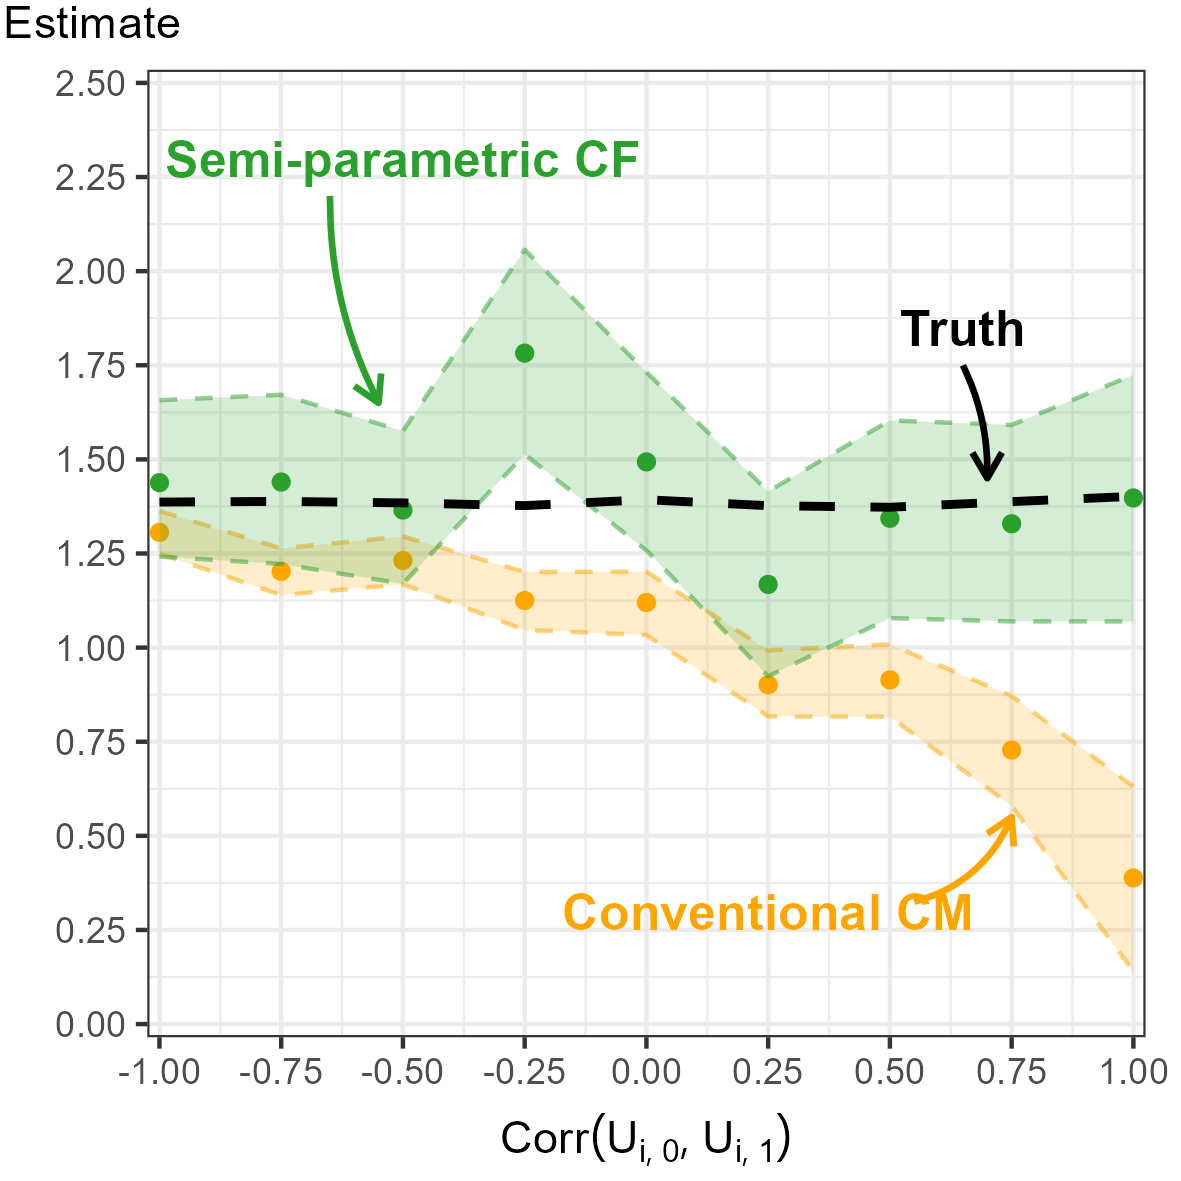
\includegraphics[width=\textwidth]{
                    ../text/sections/figures/rho-directeffect-bias.png}
            \end{subfigure}
            \begin{subfigure}[c]{0.525\textwidth}
                \centering
                \caption{AIE.}
                \vskip-0.25cm
                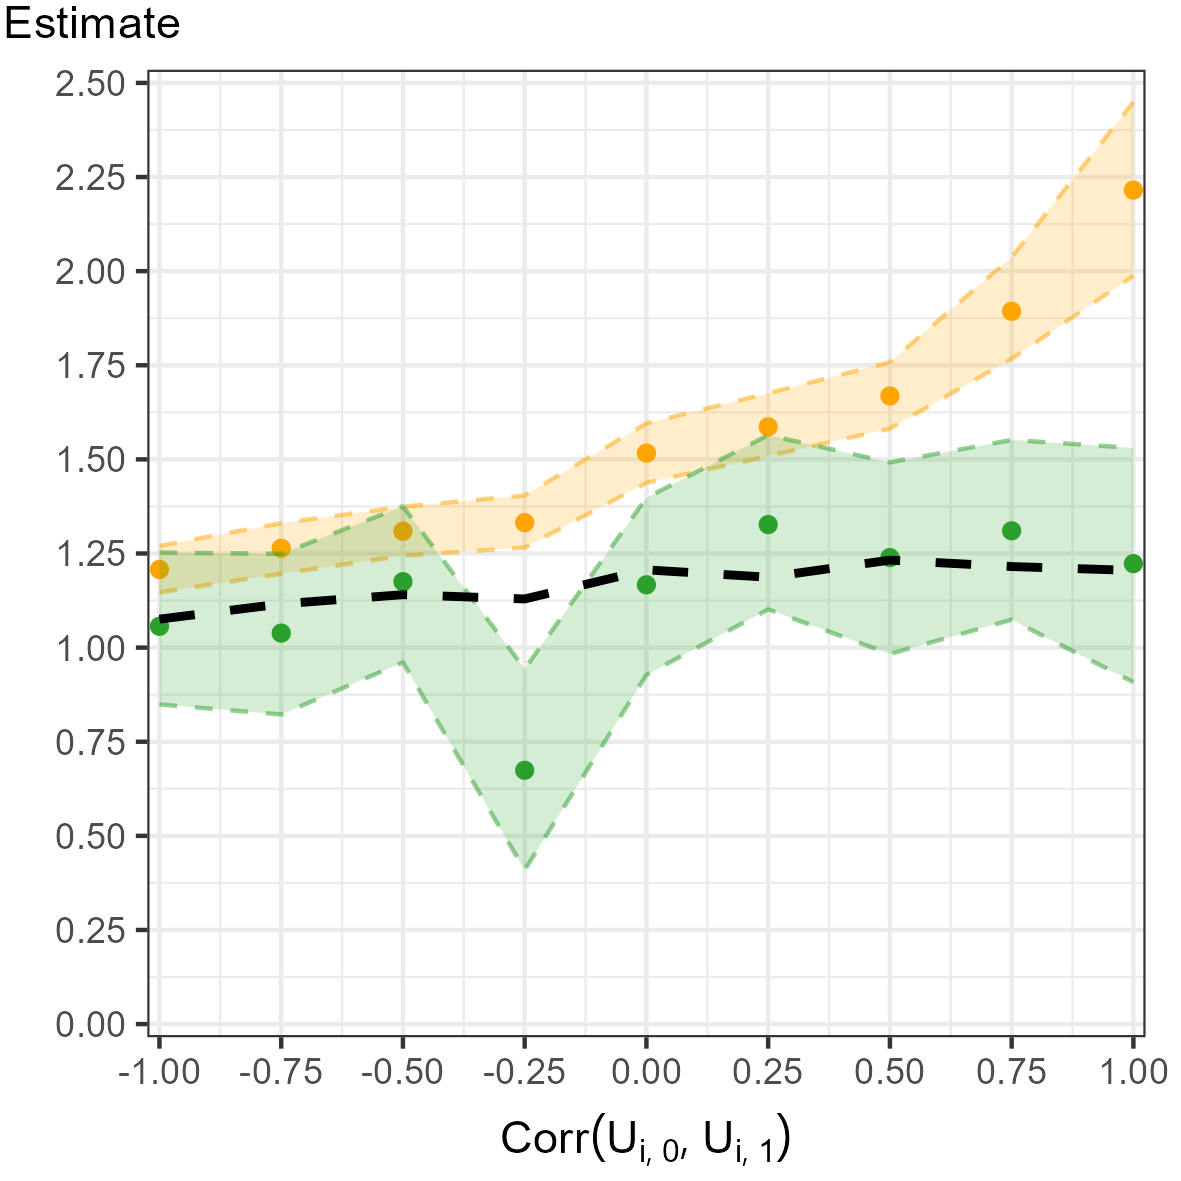
\includegraphics[width=\textwidth]{
                    ../text/sections/figures/rho-indirecteffect-bias.png}
            \end{subfigure}
        \end{figure}
    }}
\end{frame}
%-------------------------------------------------------------------------------
\begin{frame}[noframenumbering]
    \frametitle{Appenidx: OHIE IV}
    \label{ohie-iv}
    IV first-stage F stat. is 124, for all categories (minus base).
    %\vskip-0.5cm
    \begin{figure}
        \centering
        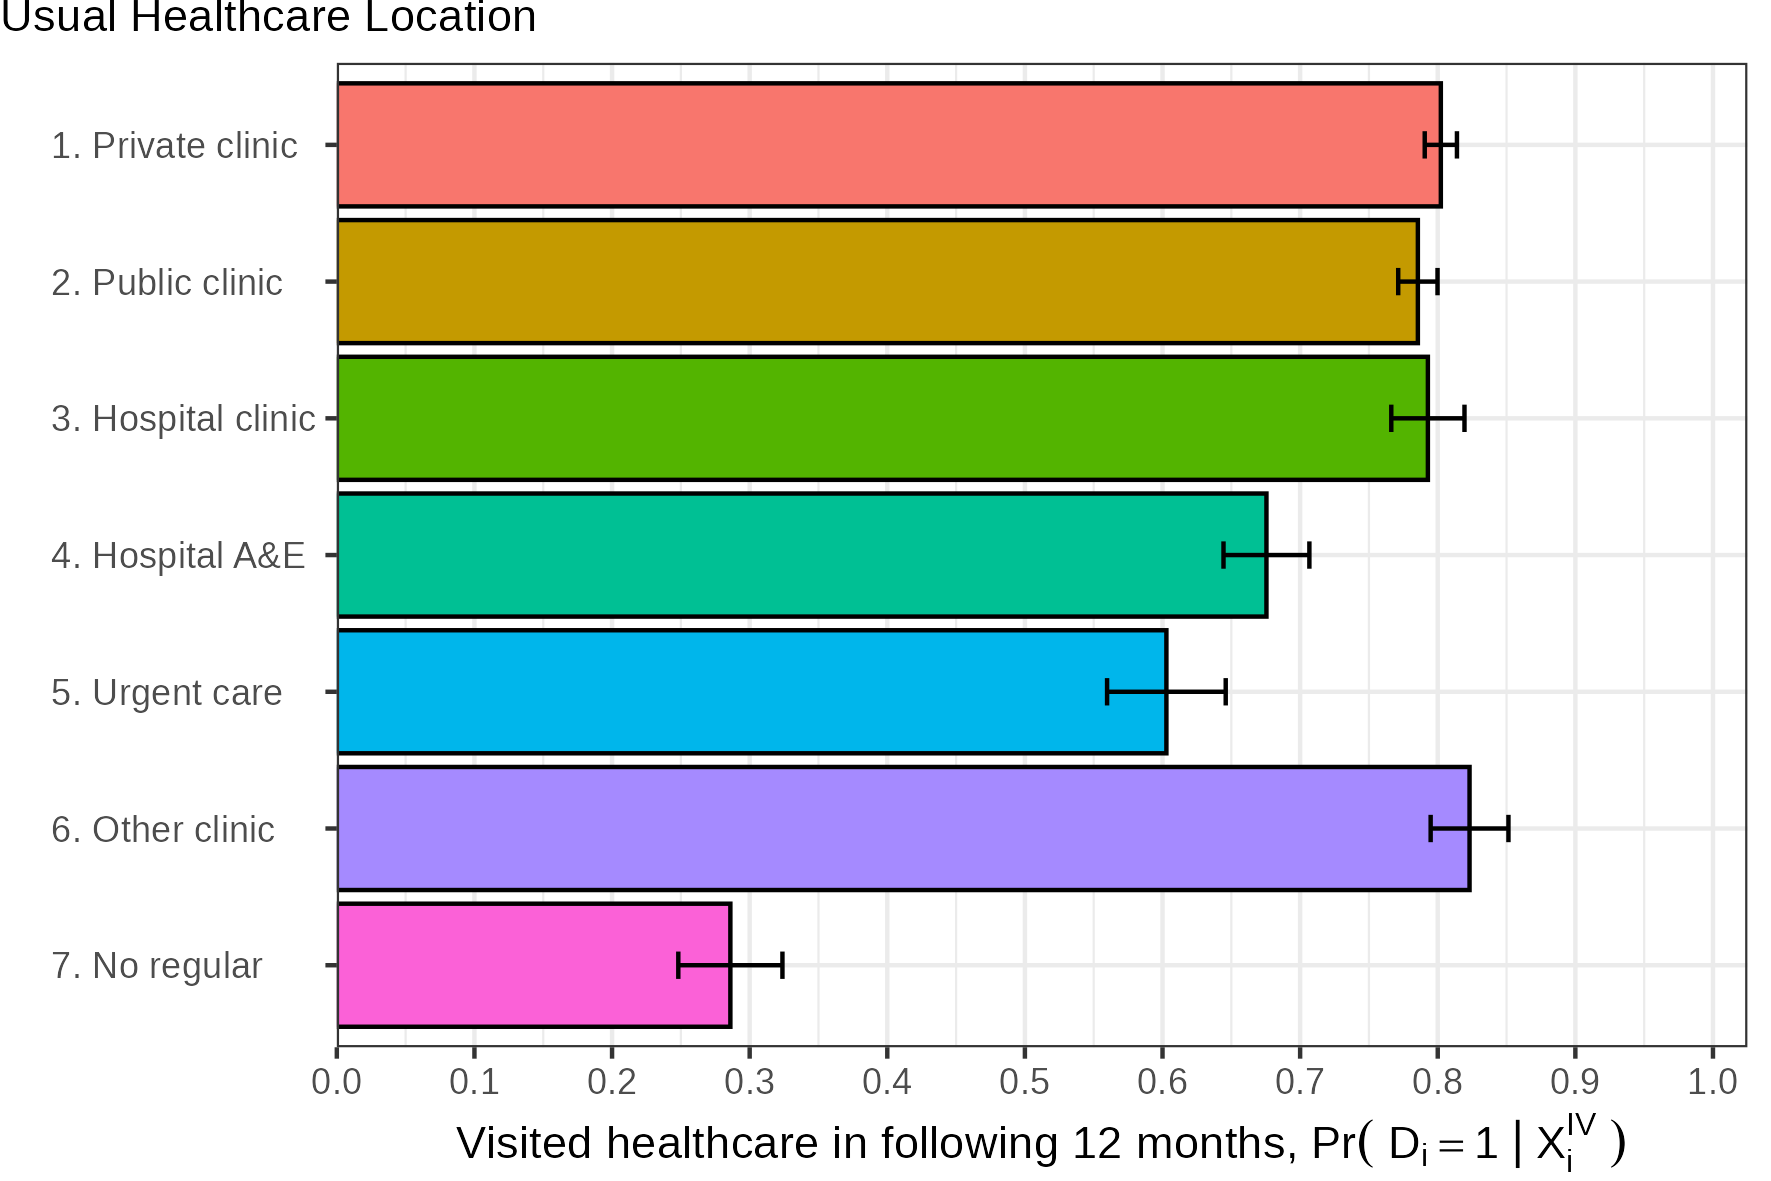
\includegraphics[height=0.7\textheight]{
            ../text/sections/figures/location-effects.png}
    \end{figure}
    Structural estimate of mediator compliers' $\textcolor{ForestGreen}{D_i} \to \textcolor{red}{Y_i}$ is \textcolor{ForestGreen}{+32.9pp (4.4)}.
\end{frame}
%-------------------------------------------------------------------------------
\end{document}
